\chapter{Special types of space}
\pagebreak[4]
\section{p112 - Exercise}
\begin{tcolorbox}
Deduce from $4.110.$ that the Gaussian curvature of a $V_2$ positive-definite metric is given by $$ G = \frac{R_{1212}}{a_{11}a_{22}-a_{12}^2}$$
\end{tcolorbox}
From p. 86 (exercise) we know that all the components of $R_{mnrs}$ can be expressed as terms of $R_{1212}$ (or vanish). \\
So by $4.110.$, 
\begin{align}
K\left({a_{11}a_{22}-a_{12}a_{21}}\right) = R_{1212}
\end{align}
and from page 96 $3.415.$ we know that for $V_2$, $K=G$. Hence,
\begin{align}
G = \frac{R_{1212}}{\left(a_{11}a_{22}-a_{12}a_{21}\right)}
\end{align}
$$\blacklozenge$$
\newpage

\section{p113 - Exercise}
\begin{tcolorbox}
Prove that, in a space $V_N$ of constant curvature $K$,$$\mathbf{4.115.}\spatie R_{mn} = -\left(N-1\right)Ka_{mn}, \quad R = -N\left(N-1\right)K$$
\end{tcolorbox}
We have
\begin{align}
R_{mn} = R^s_{.mns} = a^{sk}R_{kmns}
\end{align}
From $4.114.$
\begin{align}
R_{kmns} &= K\left(a_{kn}a_{ms}-a_{ks}a_{mn}\right)\\
&= K \left(\underbrace{\delta^s_n a_{ms}}_{a{mn}}-Na_{mn}\right)\\
&= K\left(1-N\right)a_{mn}
\end{align}
and 
\begin{align}
R &= R^n_{.n}\\
&= a^{kn}R{kn}\\
&= -\underbrace{a^{kn}a_{kn}}_{N}\left( N-1 \right)K\\
&= -N\left( N-1 \right)K
\end{align}
$$\blacklozenge$$
\newpage

\section{p113 - Clarification}
\begin{tcolorbox}
$$\mathbf{4.117.}\spatie \frac{\delta^2 \eta^r}{\delta s^2} + \epsilon K\eta^r =0$$
\end{tcolorbox}
We have
\begin{align}
R^r_{.smn} &= a^{rk} R_{ksmn}\\
\text{(4.114)}\Rightarrow \spatie &= a^{rk} K\left(a_{km}a_{sn}-a_{kn}a_{sm}\right)\\
&= K\left(\delta^r_m a_{sn}-\delta^r_n a_{sm}\right)
\end{align}
\begin{align}
\text{(3.311) and (3)}\spatie 0 &=\frac{\delta^2 \eta^r}{\delta s^2} +  K\left(\delta^r_m a_{sn}-\delta^r_n a_{sm}\right)p^s\eta^m p^n\\
\Leftrightarrow\spatie 0 &=\frac{\delta^2 \eta^r}{\delta s^2} +  K\left(\delta^r_m \eta^m \underbrace{a_{sn}p^s p^n}_{=\epsilon}-\delta^r_n \underbrace{a_{sm}p^s\eta^m}_{=0} p^n\right)\\
\Leftrightarrow\spatie 0 &=\frac{\delta^2 \eta^r}{\delta s^2} +  K\epsilon\underbrace{\delta^r_m \eta^m}_{=\eta^r} \\
\Leftrightarrow\spatie 0 &=\frac{\delta^2 \eta^r}{\delta s^2} +  K\epsilon\eta^r
\end{align}
$$\blacklozenge$$
\newpage

\section{p114 - Clarification}
\begin{tcolorbox}
$$\mathbf{4.118.}\spatie \dv[2]{\left(X_r\eta^r\right)}{s} + \epsilon K\left(X_r\eta^r\right) =0$$
\end{tcolorbox}
We know that $\frac{\delta X_r}{\delta s} = 0$ (parallel transport)
\begin{align}
\frac{\delta \left(X_r\eta^r\right)}{\delta s}&= \eta^r\underbrace{\frac{\delta X_r}{\delta s}}_{=0}+X_r\frac{\delta \eta^r}{\delta s}\\
\Rightarrow\spatie \frac{\delta^2 \left(X_r\eta^r\right)}{\delta s}&= \underbrace{\frac{\delta X_r}{\delta s}}_{=0}\frac{\delta \eta^r}{\delta s}+X_r\frac{\delta^2 \eta^r}{\delta s^2}\\
\Rightarrow\spatie X_r\frac{\delta^2 \eta^r}{\delta s^2}&= \frac{\delta^2 \left(X_r\eta^r\right)}{\delta s^2}\\
\text{but}\spatie \frac{\delta^2 \left(X_r\eta^r\right)}{\delta s^2} &=  \dv[2]{X_r\eta^r}{s} \quad \text{ as } X_r\eta^r \text{ is an invariant}\\
\Rightarrow X_r\frac{\delta^2 \eta^r}{\delta s^2}&=\dv[2]{X_r\eta^r}{s}\\
\text{and so}\spatie \frac{\delta^2 \left(\eta^r\right)}{\delta s^2}X_r + \epsilon K\left(X_r\eta^r\right) &= \dv[2]{X_r\eta^r}{s}+ \epsilon K\left(X_r\eta^r\right) = 0
\end{align}
$$\blacklozenge$$
\newpage

\section{p115 - Exercise}
\begin{tcolorbox}
By taking an orthonormal set of $N$ unit vectors propagated parallely along the geodesic, deduce from $4.120a$ that the magnitude $\eta$ of the vector $\eta^r$ is given by $$ \eta = C\left|\sin \left(s\sqrt{\epsilon K}\right)\right|$$ where $C$ is a constant.
\end{tcolorbox}
We have by $4.120a$
\begin{align}
X_r \eta^r &= A\sin \left(s\sqrt{\epsilon K}\right)
\end{align}
We choose $N$ different $X^{(k)}_r$ $(k= 1,2,\dots, N)$ which are orthonormal.
Applying $(1)$ $N$ times with the different $X^{(k)}_r$ $(k= 1,2,\dots, N)$, we get
\begin{align}
X^{(k)}_r \eta^r &= A^{(k)}\sin \left(s\sqrt{\epsilon K}\right)
\end{align}
But as the $X^{(k)}_r$ are orthonormal and are used as a basis at the considered point of the geodesic we have 
\begin{align}
X^{(k)}_r &= \delta^k_r
\end{align}
So, $(2)$ becomes
\begin{align}
\eta^k &= A^{(k)}\sin \left(s\sqrt{\epsilon K}\right)
\end{align}
which are the components of the displacement vector in the orthonormal basis. By $\mathbf{2.301.}$ :
\begin{align}
Y^2 &= \epsilon a_{mn} Y^m Y^n\\
\Rightarrow \spatie \eta^2 &= \epsilon a_{mn} A^{(m)} A^{(n)}\sin^2 \left(s\sqrt{\epsilon K}\right)\\
\Rightarrow \spatie \eta &= C\left|\sin \left(s\sqrt{\epsilon K}\right)\right|\\
\text{with}\spatie C&= \sqrt{\left|\epsilon a_{mn} A^{(m)} A^{(n)}\right|}
\end{align}
$$\blacklozenge$$
\newpage

\section{p118 - Exercise}
\begin{tcolorbox}
Examine the limit of the form $\mathbf{4.130}$ as $R$ tends to infinity, and interpet the result.
\end{tcolorbox}
We have $$\mathbf{4.130.}\spatie ds^2 = dr^2+R^2\sin^2\left(\frac{r}{R}\right)\left(d\theta^2 + \sin^2\theta d\phi^2\right)$$
But $\sin \epsilon \approx \epsilon$ for $\epsilon  \ll 1$. So
\begin{align}
 \lim_{R\rightarrow \infty} ds^2 &= dr^2+R^2\left(\frac{r}{R}\right)^2\left(d\theta^2 + \sin^2\theta d\phi^2\right)\\
 &= dr^2+\left(r d\theta^2 \right) + \left(r\sin\theta d\phi\right)^2
 \end{align}
 This is the metric form for an Euclidean 3-space with spherical polar coordinates (see $\mathbf{2.532.}$ page 54).
$$\blacklozenge$$
\newpage

\section{p119 - Exercise}
\begin{tcolorbox}
Show that a transformation of a homogeneous coordinate system  into another homogeneous system is necessarily linear. (Use the transformation equation $\mathbf{2.507}$ for Christoffel symbols, noting that all Christoffel symbols vanish  when the coordinates are homogeneous).
\end{tcolorbox}
By $2.507$ we have the transformation rule 
\begin{align}
\Gamma^{'a}_{bc} = \Gamma^{r}_{mn}\partial_r z^a\partial_b z^m \partial_c z^n + \partial_r z^a\frac{\partial^2 z^r}{\partial z^b \partial z^c} 
\end{align}
But, as both coordinate system are homogeneous, all Christoffel symbols vanish and so
\begin{align}
\Gamma^{'a}_{bc} = \partial_r z^a\frac{\partial^2 z^r}{\partial z^b \partial z^c} &=0\\
\Rightarrow \spatie \partial_r z^a\frac{\partial^2 z^r}{\partial z^b \partial z^c} &=0
\end{align}
As the Jacobian can't vanish the possibility of having $\partial_r z^a=0$ $\forall a, r$ is excluded. Hence we must have $\frac{\partial^2 z^r}{\partial z^b \partial z^c} =0$. And have a linear solution of the form
\begin{align}
z^r = A_k z^{'k}+C
\end{align}
$$\blacklozenge$$
\newpage

\section{p120 - Exercise}
\begin{tcolorbox}
If $z_r, z^{'}_r$ are two systems of rectangular Cartesian coordinates in Euclidean 3-space, what is the geometrical interpretation of the constants in $\mathbf{4.204}$ and of the orthogonality conditions $\mathbf{4.209}$ ?
\end{tcolorbox}
We have 
\begin{align}
z^{'}_m &= A_{mn}z_n+A_m 
\end{align}
As we assume that the Jacobian of the transformation does not vanish and thus the mapping is bijective, in an Euclidean 3-space $A_m$ will perform a $\mathit{translation}$ while $A_{mn}$ can be interpreted as a combination rotation/reflection/stretching/contraction/shearing. I.e. the mapping is an $\mathit{affine}$ transformation.\\
The condition $\mathbf{4.209}$ restricts the action of $A_{mn}$ to a combination of rotation/reflection. Indeed, a rotation/reflection can be represented by $R= R_x\left(\gamma\right) \circ R_y\left(\beta\right)\circ  R_z\left(\alpha\right)$ with 
\begin{align}
R_x = \begin{pmatrix}
\pm 1&0  &0  \\
0&\cos\gamma & -\sin\gamma \\
 0&\sin\gamma & \cos\gamma   \\
\end{pmatrix}
R_y = \begin{pmatrix}
\cos\beta & 0& -\sin\beta \\
 0& \pm 1&0 \\
 \sin\beta & 0& \cos\beta\\
\end{pmatrix}
R_z = \begin{pmatrix}
\cos\alpha & -\sin\alpha  & 0 \\
 \sin\alpha & \cos\alpha  & 0 \\
  0&0  & \pm 1 \\
\end{pmatrix}
\end{align}
Note that for every axis, $R_k^{T} R_k^{} = \mathbb{I}_3$.\\
Be $A_{mn} = R_x\left(\gamma\right) \circ R_y\left(\beta\right)\circ  R_z\left(\alpha\right)$
We have by $\mathbf{4.209}$, $A_{mq}A_{mq}= \delta_{pq}$ which can be expressed as 
\begin{align}
A^{T}A &= \mathbb{I}_3\\
\Rightarrow \spatie \mathbb{I}_3 &= \left( R_x R_y R_z\right)^T R_xR_yR_z\\
&=  \underbrace{R_z^T \underbrace{R_y^T\underbrace{R_x^TR_x}_{= \mathbb{I}} R_y}_{= \mathbb{I}}R_z}_{= \mathbb{I}_3}
\end{align}
The identity yields, and interpret the coefficients of the orthogonal transformation as an Euclidean orthogonal transformation. 
$$\blacklozenge$$
\newpage

\section{p123 - Clarification}
\begin{tcolorbox}
If $A_{n}A_{n} =0$ it follows from $\mathbf{2.445}$ and $\mathbf{2.446}$ that the straight line is a geodesic null line.
\end{tcolorbox}
We have 
\begin{align}
\text{(2.446)}\spatie & a_{mn}\dv{x^m}{u}\dv{x^n}{u}=0 \spatie \dv{x^m}{u}= \dv{z_m}{u} = A_m\\
\text{(4.215)}\spatie & a_{mn}=\delta_{mn}\\
\text{(1),(2) \ }\Rightarrow \spatie &\delta_{mn}\dv{z_m}{u}\dv{z_n}{u}=0\\
\Rightarrow \spatie &A_nA_n=0
\end{align}
$$\blacklozenge$$
\newpage


\section{p123 - Clarification}
\begin{tcolorbox}
It is easy to see ... viz., $$\mathit{the \ straight \ line \ joining \ any \ two \ points \ in \ a \ plane \ lies \ entirely \ in \ the \ plane.}$$ 
\end{tcolorbox}
The plane is identified by 
\begin{align}
A_n z_n+B=0
\end{align}
and a line by
\begin{align}
z_n = C_nu+D_n
\end{align}
Take two points at $u=0$ and $u=p$ lying in the plane:
\begin{align}
& \left\{ \begin{array}{l}
A_nC_np+A_nD_n+B=0\\
A_nD_n+B=0
\end{array} \right.\\
\Rightarrow\spatie & \left\{ \begin{array}{l}
A_nC_np=0\\
A_nD_n+B=0
\end{array} \right.
\end{align}
And as $p\neq 0 \ \Rightarrow A_nC_n = 0$. So for any arbitrary $u$ of this line we have
\begin{align}
\underbrace{A_nC_n}_{=0}u+\underbrace{A_nD_n}_{=0}+B=0
\end{align}
hence, all points of the line lie in the plane.
$$\blacklozenge$$
\newpage


\section{p123 - Exercise}
\begin{tcolorbox}
Show that a one-flat is a straight line.
\end{tcolorbox}
A one-flat means $(N-1)$ equations 
\begin{align}
A^{(k)}_nz_n + B^{(k)} =0 \quad k=1,\dots,N-1\quad n= 1,\dots,N
\end{align}
This is a set of $(N-1)$ linear equation in $N$ unknown $z_n$. So we have one degree of freedom.\\
E.g. put $z_N=u$ with u the free parameter. then,
\begin{align}
A^{(k)}_{\alpha}z_{\alpha}+ A^{(k)}_{N}u+ B^{(k)} =0 \quad \alpha=1,\dots,N-1
\end{align}
If $detA^{(k)}_{\alpha} \neq0$ we get a solution of the et of equation
\begin{align}
Az&=B \quad\text{with}\quad B \text{ a linear function in } u\\
\Rightarrow\spatie z_m&= \left(A^{-1}B\right)_m
\end{align}
with $\left(A^{-1}B\right)_m$ of the form $C_mu+D_m$
$$\blacklozenge$$
\newpage

\section{p126 - Exercise}
\begin{tcolorbox}
Show that the null cone with vertex at the origin in space-time has the equation $$\mathbf\spatie y^2_1+y^2_2+y^2_3-y^2_4=0$$
Prove that this null cone divides space-time into three regions such that \\
$\mathit{a.}$ Any two points (events) both lying in one region can be joined by a continuous curve which does not cut the null cone.\\
$\mathit{b.}$ All continuous curves joining two given points (events) which lie in different regions, cut the null cone.\\
Show further that the three regions may be further classified into past, present, and future as follows: If $A$ and $B$ are any two points in the past, then the straight segment $AB$ lies entirely in the past. If $A$ and $B$ are any two points in the future, then the straight segment $AB$ lies entirely in the future. If $A$ is any point in the present, there exist at least one point $B$ in the present that the straight segment $AB$ cuts the null cone.
\end{tcolorbox}

We first prove 
$$\mathbf\spatie y^2_1+y^2_2+y^2_3-y^2_4=0$$
The null geodesic equations:
\begin{align}
& \left\{ \begin{array}{l}
\frac{\delta^2 x^r}{\delta u^2} = \dv[2]{x_r}{u} =0 \quad \text{ as we use homogeneous coordinates}\\\\
a_{mn} \dv{x_m}{u}\dv{x_n}{u}=0\\
\end{array} \right.\\
\Rightarrow \spatie & \left\{ \begin{array}{l}
x_r = A_ru+B_r\quad \text{( put } B_r=0 \text{ by aqequate choice of the origin )} \\\\
A_1^2+A_2^2+A_1^2+A_3^2-A_4^2=0\\
\end{array} \right.\\
\Rightarrow \spatie &\frac{\left((x_1)^2+(x_2)^2+(x_3)^2-(x_4)^2\right)}{u^2} = 0\quad \text{ for } u\neq 0\\
\Rightarrow \spatie &(x_1)^2+(x_2)^2+(x_3)^2-(x_4)^2 = 0
\end{align}
$$\lozenge$$
About the existence of three regions. First let's investigate the case in a $V_3$ space-time manifold in order to have a more intuitive grasp.\\
Consider a family of events $(p_1,p_2,u)$ with $u\in\left(-\infty,\infty\right)$ (see the line $P^{'}P^{"}$ in figure 1.1.)
\begin{figure}[H]
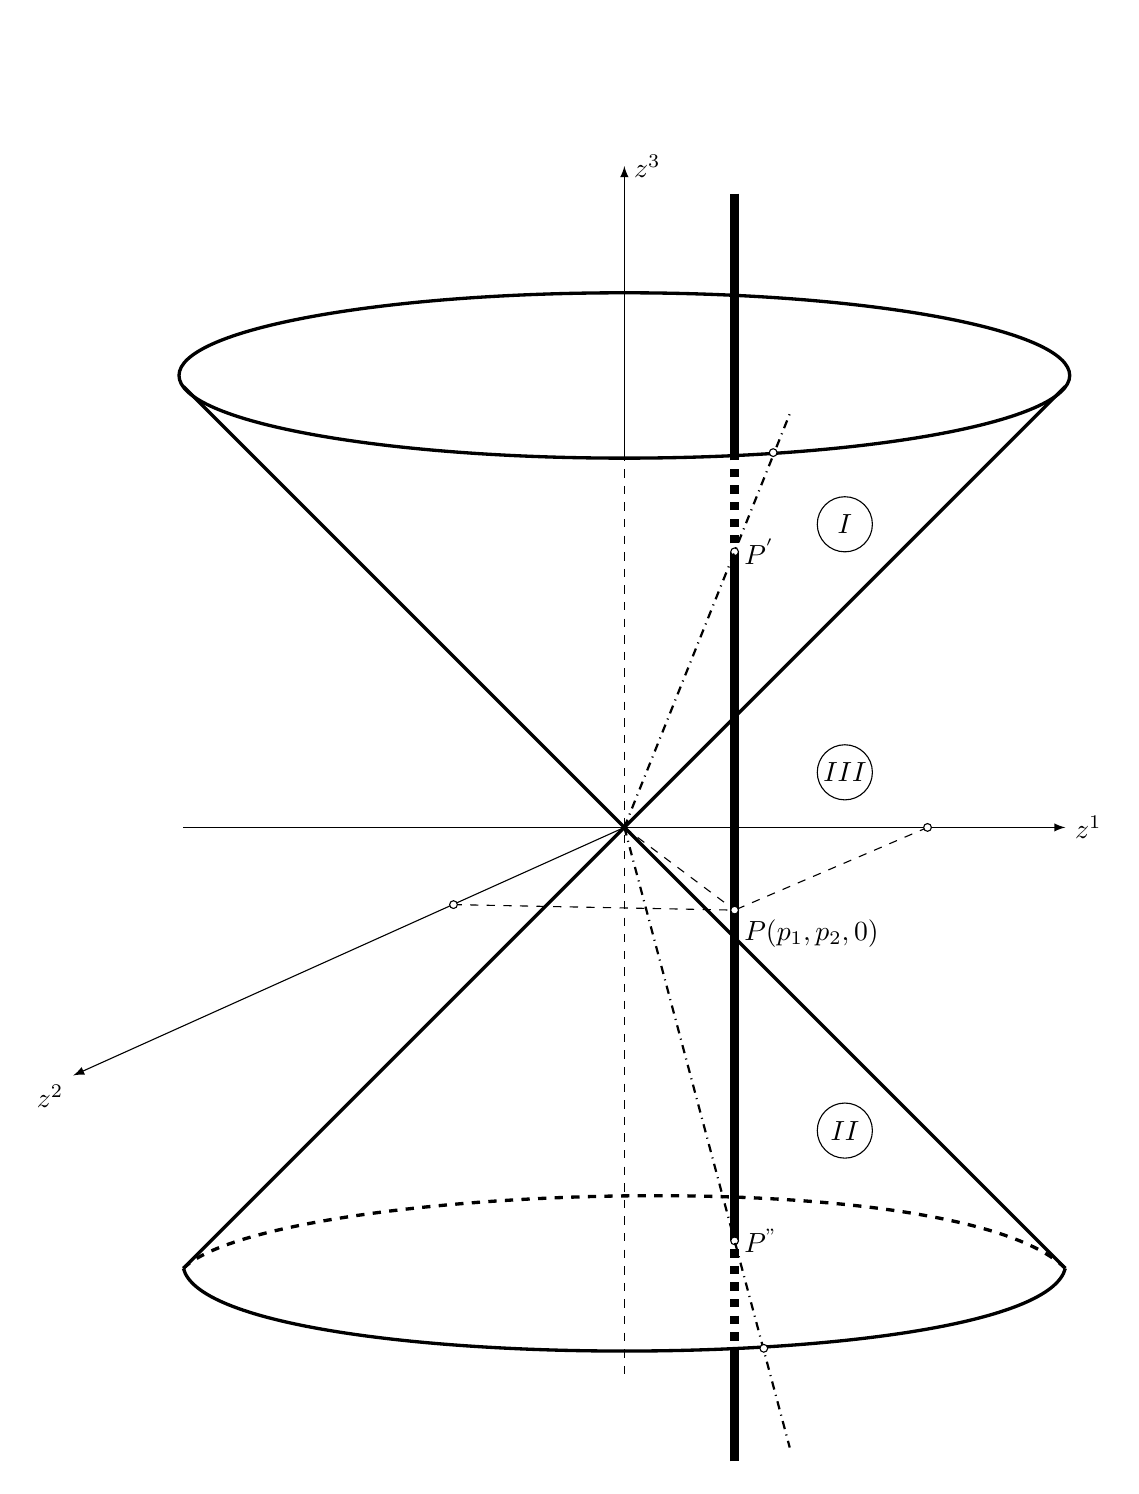
\begin{tikzpicture}[scale=0.70]
\coordinate (v1) at (-8,-0);
\coordinate (v2) at (8,-0) ;
\coordinate (v3) at (0,12) {};
\coordinate (v4) at (0,6.8) {};
\coordinate (v5) at (8,8) {};
\coordinate (v6)  at (0,0) {};
\coordinate (v7) at (-8,-8) {};
\coordinate (v8) at (8,-8) {};
\coordinate (v9) at (-8,8) {};
\coordinate (v10) at (-0,-10) {};
\coordinate (v11)  at (-10,-4.5) {};
\draw[-{latex}]  (v1)-- (v2)node[right] {$z^1$};
\draw  [-{latex}](v4)-- (v3)node[right] {$z^3$};
\draw  [-{latex}](v6)-- (v11)node[{anchor=north east}] {$z^2$};
\draw  [dashed](v4)-- (v10);
\draw[very thick]  (0,8.2) ellipse (8.08 and 1.5);
\draw [very thick] (v6) -- (v5);
\draw [very thick] (v7) -- (v6);
\draw  [very thick](v6) -- (v8);
\draw  [very thick](v6) -- (v9);
\draw[very thick] (-8,-8) .. controls (-7.5,-10) and (7.5,-10) .. (8,-8);
\draw [very thick, dashed,](-8,-8) .. controls (-6.5,-6.5) and (6,-6) .. (8,-8);

\coordinate (p0) at (-3.1,-1.4) {} {};
\coordinate (p1) at (2,-1.5) {} {};
\coordinate (p2) at (2,5) {} {};
\coordinate (p3) at (2,-7.5) {} {};
\coordinate (p4) at (5.5,0) {};
\draw [dashed, thin] (p0) -- (p1);
\draw [dashed, thin] (p4) -- (p1);
\draw [dashed, thin] (v6) -- (p1);
\draw [line width=3] (p2) -- (p1);
\draw [line width=3] (p2) -- (p3);
\coordinate (p5) at (2,6.7) {};
\coordinate (p6) at (2,-9.5) {};
\coordinate (p7)at (2,11.5) {};
\coordinate (p8)  at (2,-11.5) {};
\draw [dashed, line width=3] (p3) -- (p5);
\draw  [dashed, line width=3] (p2) -- (p6);
\draw [ line width=3] (p7) -- (p5);
\draw[ line width=3] (p8) -- (p6);
\draw[fill=white](p0) circle(2pt);
\draw[fill=white](p4) circle(2pt);
\draw[fill=white](p3) circle(2pt)node[{anchor=west }] {$P^{"}$};
\draw[fill=white](p2) circle(2pt)node[{anchor=west }] {$P^{'}$};
\draw[fill=white](p1) circle(2pt)node[{anchor=north west }] {$P(p_1,p_2,0)^{}$};
\coordinate (p9)  at (1.5*2,-1.5*7.5) {};
\coordinate (p10)  at (1.5*2,1.5*5) {};
\draw  [dashdotted,thick](v6) edge (p9);
\draw  [dashdotted,thick](v6) edge (p10);
\coordinate (t1) at (4,5.5) {};
\coordinate (t2) at (4,1) {} ;
\coordinate (t3) at (4,-5.5) {};
\draw[fill=black](t1)node[] {$I$};
\draw[fill=black](t2)node[] {$III$};
\draw[fill=black](t3)node[] {$II$};
\coordinate (t4) at (2.7,6.8) {};
\coordinate (t5) at (2.53,-9.45) {};
\draw[fill=white](t4) circle(2pt);
\draw[fill=white](t5) circle(2pt);

\draw  (t1) ellipse (0.5 and 0.5);
\draw  (t2) ellipse (0.5 and 0.5);
\draw  (t3) ellipse (0.5 and 0.5);
\draw  (-1.5,14.5) ellipse (0 and 0);
\end{tikzpicture}
\caption{Regions delimited by the light cone in a $V_3$ space-time manifold}
\label{fig:fig_p96_3415_a}
\end{figure}
Be $R^2 = y_1^2 +y_2^2$. The light cone has the the equation $R^2- y_3^2=0$. Only the events at $ u_0 = \pm R(p_1,p_2)$ will lie on the light-cone.\\
We can distinguish three regions:\\
Region I where $u > u_0 = R$: the events $(p_1,p_2,u)$ will lie on the line above point $P^{'}$.\\
Region II where $ u < -u_0 = -R$: the events $(p_1,p_2,u)$ will lie on the line below point $P^{"}$.\\
Region III where $ -R= -u_0 < u < u_0 = R$: the events $(p_1,p_2,u)$ will lie on the segment $P^{'}P^{"}$.\\
Let's generalize this now for a $V_4$ space-time manifold.\\
Put $R^2 = (y_1)^2+(y_2)^2+(y_3)^2$ and consider $\phi(y_1,y_2,y_3,y_4)= (y_1)^2+(y_2)^2+(y_3)^2-(y_4)^2$ so $\phi(y_1,y_2,y_3,y_4)= R^2-(y_4)^2$.\\
For $\phi=0$ we lie on the light-cone.\\
For $\phi>0 \quad\Rightarrow R^2 > y_4^2$ and so $-R<y_4<R$ defines one region (region III).\\
For $\phi<0 \quad\Rightarrow R^2 < y_4^2$ and so   $y_4>R$ and $y_4<-R$ define two  regions (region I and II).\\$$\lozenge$$\\\\
\textbf{We now show statement $\mathit{a.}$ of the exercise.}\\
Consider $2$ events $P_0,\ P_1$ with coordinates $(y_1^{(0)},y_2^{(0)},y_3^{(0)},y_4^{(0)})$ and $(y_1^{(1)},y_2^{(1)},y_3^{(1)},y_4^{(1)})$  and a curve defined by 
\begin{align}y_i= \pm\sqrt{\left(\left(y_i^{(1)}\right)^2-\left(y_i^{(0)}\right)^2\right)u + \left(y_i^{(0)}\right)^2}\spatie u\in \left[0,1\right]
\end{align}
where the $\pm$ is chosen so that $y_i(0) = y_i^{(0)}$ and $y_i(1) = y_i^{(1)}$ and that the sign only changes when $y_i(u)=0$ and $sign\left(y_i^{(0)}\right) \neq sign\left(y_i^{(1)}\right)$. Such curve will be continuous.
Put
\begin{align}
R^2&= \left(y_1\right)^2+\left(y_2\right)^2+\left(y_3\right)^2\\
{R_{0}}^2&= \left(y^0_1\right)^2+\left(y^0_2\right)^2+\left(y^0_3\right)^2\\
{R_{1}}^2&= \left(y^1_1\right)^2+\left(y^1_2\right)^2+\left(y^1_3\right)^2
\end{align}
For the points on the curve defined by  (5), $R^2$ can then be written as 
\begin{align}
R^2&= \left(R_1^2-R_0^2\right)u+R_0^2
\end{align}
Be $\phi(u)= R^2-y_4^2$.\\
\textbf{Case a1: $P_0, P_1$ both lie in region I or both in region II.} Then,\\
\begin{align}
\phi(u) & < 0\quad \forall \ u\in \left[0,1\right]\\
\Rightarrow\quad R_0^2 < (y_4^{0})^2 \quad &\wedge \quad  R_1^2 < (y_4^{1})^2 \\ \text{ with }   (y_4^{0}>0 \  \wedge \ y_4^{1}>0)\text{ in Region I}\quad &\vee \quad (y_4^{0}<0\quad \wedge \quad y_4^{1}<0)  \text{ in Region II}
\end{align}
Then, $$\cancel{\exists } \  u \in \left[0,1\right]: \phi(u)=0$$
Indeed,
\begin{align}
\phi(u) &= \left(R_1^2-R_0^2\right)u+R_0^2 + \left(\left(y_4^{(0)}\right)^2   -\left(y_4^{(0)}\right)^2 \right)u -\left(y_4^{(0)}\right)^2\\
\phi(u)=0\spatie \Rightarrow u&= -\frac{R_0^2- \left(y_4^{(0)}\right)^2}{R_1^2-R_0^2  -\left(y_4^{(1)}\right)^2  +\left(y_4^{(0)}\right)^2}
\end{align}
Let's simplify notationally the last equation. Put $R_0^2- \left(y_4^{(0)}\right)^2=-\tau $ and $R_1^2- \left(y_4^{(1)}\right)^2=-\sigma$ with both $\tau, \sigma > 0$. $(14)$ can be written as
\begin{align}
u&=\frac{\tau}{\tau-\sigma}\\
 &=\frac{1}{1-\frac{\sigma}{\tau}}\\
\Rightarrow\spatie \left|u\right| & > 1 \spatie \text{ as } \frac{\sigma}{\tau} >0
\end{align}
Note, that in the case $\tau=\sigma$ we have $\phi(u)= \tau = \text{ constant}$ and can't reach $0$.
So, there exist no $u\in\left[0,1\right]$ for which $\phi(u)=0$ and the curve does not intersect the null cone.\\\\
\textbf{Case a2: $P_0, P_1$ both lie in region III.} Then,\\
\begin{align}
\phi(u) & > 0\quad \forall \ u\in \left[0,1\right]\\
\Rightarrow\quad R_0^2 > (y_4^{0})^2 \quad &\wedge \quad  R_1^2 > (y_4^{1})^2 
\end{align}
Then, $$\cancel{\exists } \  u \in \left[0,1\right]: \phi(u)=0$$
Indeed,
Let's simplify  notationally the  equation (14) by now by puting $R_0^2- \left(y_4^{(0)}\right)^2=\tau $ and $R_1^2- \left(y_4^{(1)}\right)^2=\sigma$ with both $\tau, \sigma > 0$. $(14)$ can be written again as
\begin{align}
u& =\frac{1}{1-\frac{\sigma}{\tau}}
\end{align}
and follow the same reasoning as in case 1.
So, there exist no $u\in\left[0,1\right]$ for which $\phi(u)=0$ and the curve does not intersect the null cone.\\\\
\\$$\lozenge$$\\\\
\textbf{We now show statement $\mathit{b.}$ of the exercise.}\\\\

\textbf{Case b1: $P_0$ lies in region I, $P_1$  lies in region II.} \\
Those two regions are separated by the $3$-flat (plane) $y_4=0$. So it's suffice that $R^2=0$ for $\phi(u)$ being zero. Hence $y_i=0$, $  i=1,2,3$, and the cruve will cut the cone at it's apex.
\\\\
\textbf{Case b2: $P_0$ lies in region I or II, $P_1$  lies in region III.} \\
We have 
\begin{align}
R_0^2 > (y_4^{0})^2\quad R_1^2 < (y_4^{1})^2
\end{align}
Put $R_0^2 - (y_4^{0})^2= \tau$ and $R_1^2 - (y_4^{1})^2 =-\sigma$ with $\tau,\sigma >0$. We get
\begin{align}
\phi(u)&=0\\
\Rightarrow \spatie u&=-\frac{\tau}{-\sigma-\tau}\\
&= \frac{1}{1+\frac{\sigma}{\tau}}
\end{align}
So, there is a solution $u\in \left[0,1\right]$ for which $\phi(u)=0$ and the curve intersects the null cone.
\\$$\lozenge$$\\\\

\textbf{We now investigate the straight segment questions.} \\
Case 1: $A$ and $B$ both lie in the the present (region I) or in the past (region II)\\
Consider $2$ events $P_0,\ P_1$ with coordinates $(y_1^{(0)},y_2^{(0)},y_3^{(0)},y_4^{(0)})$ and $(y_1^{(1)},y_2^{(1)},y_3^{(1)},y_4^{(1)})$  and a segment  defined by 
\begin{align}y_i= \left(y_i^{(1)}-y_i^{(0)}\right)u + y_i^{(0)}\spatie u\in \left[0,1\right]
\end{align}
Be $\phi(u)= y_1^2+y_2^2+y_3^2-y_4^2$.\\
Then,
 \begin{align}
\phi(u) &= \left\{\begin{array}{l} \ \ \left[\left(y_1^{(1)}-y_1^{(0)}\right)u + y_1^{(0)}\right]^2\\
+\left[\left(y_2^{(1)}-y_2^{(0)}\right)u + y_2^{(0)}\right]^2\\
+\left[\left(y_3^{(1)}-y_3^{(0)}\right)u + y_3^{(0)}\right]^2\\
-\left[\left(y_4^{(1)}-y_4^{(0)}\right)u + y_4^{(0)}\right]^2\\
\end{array}\right.\\
&= \left\{\begin{array}{l} \ \ 
\left(y_1^{(1)}\right)^2 u^2+\left(y_1^{(0)}\right)^2 u^2 - 2y_1^{(1)}y_1^{(0)}u^2 + 2y_1^{(1)}y_1^{(0)}u-  2\left(y_1^{(0)}\right)^2 u+ \left(y_1^{(0)}\right)^2\\
+\left(y_2^{(1)}\right)^2 u^2+\left(y_2^{(0)}\right)^2 u^2 - 2y_2^{(1)}y_2^{(0)}u^2 + 2y_2^{(1)}y_2^{(0)}u-  2\left(y_2^{(0)}\right)^2 u+ \left(y_2^{(0)}\right)^2\\
+\left(y_3^{(1)}\right)^2 u^2+\left(y_3^{(0)}\right)^2 u^2 - 2y_3^{(1)}y_3^{(0)}u^2 + 2y_3^{(1)}y_3^{(0)}u-  2\left(y_3^{(0)}\right)^2 u+ \left(y_3^{(0)}\right)^2\\
-\left(y_4^{(1)}\right)^2 u^2-\left(y_4^{(0)}\right)^2 u^2 + 2y_4^{(1)}y_4^{(0)}u^2 - 2y_4^{(1)}y_4^{(0)}u+  2\left(y_4^{(0)}\right)^2 u- \left(y_4^{(0)}\right)^2\\
\end{array}\right.
\end{align}
Put $\phi_0 = \left(y_1^{(0)}\right)^2+\left(y_2^{(0)}\right)^2+\left(y_3^{(0)}\right)^2-\left(y_4^{(0)}\right)^2$ and $\phi_1 = \left(y_1^{(1)}\right)^2+\left(y_2^{(1)}\right)^2+\left(y_3^{(1)}\right)^2-\left(y_4^{(1)}\right)^2$. \\
Then,
\begin{align}
\phi(u)= \left\{\begin{array}{l} \ \ 
\phi_1u^2+\phi_0u^2-2\left(y_1^{(1)}y_1^{(0)}+y_2^{(1)}y_2^{(0)}+y_3^{(1)}y_3^{(0)}-y_4^{(1)}y_4^{(0)}\right)u^2 \\
-2\phi_0 u + 2 \left(y_1^{(1)}y_1^{(0)}+y_2^{(1)}y_2^{(0)}+y_3^{(1)}y_3^{(0)}-y_4^{(1)}y_4^{(0)}\right)u\\
+\phi_0
\end{array}\right.
\end{align}
Let's put $\kappa = y_1^{(1)}y_1^{(0)}+y_2^{(1)}y_2^{(0)}+y_3^{(1)}y_3^{(0)}-y_4^{(1)}y_4^{(0)}$, we get the expression
\begin{align}
\phi(u)&= 
\left(\phi_1 +\phi_0-2\kappa\right) u^2 + 2 \left(\kappa- \phi_0\right)u
+\phi_0
\end{align}


The function $\phi(u)$ is a parabola. 
\begin{figure}[H]%
    \centering
    \subfloat[]{
       


            
\begin{tikzpicture} [scale=0.5,c/.style={insert path={circle[radius=3pt]}}] 
\pgfplotsset{every axis/.append style={
		scale=1,
		axis lines=center,
		axis on top,
		xlabel={$u$},
		ylabel={$\phi(u)$},
               axis x line=middle,    % put the x axis in the middle
               axis y line=middle,    % put the y axis in the middle
               %x axis line style={-latex, ultra thin}, % arrows on the axis
               y axis line style={draw opacity=1},
                x axis line style={draw opacity=1},
            }}
     
					
	\tikzmath{\u=5;\a=0.2;\b=2*\a;\d=-1;}
	 \u,\a, \b,\d;
    \pgfplotsset{ };
    
    \pgfplotsset{compat=1.12};
		\def\r{3};
		\def\H{1.0};  
		\def\s{0.123};
	\begin{axis}
		[
		xmin=-3,
		xmax=3,
		ymin=-1.4,
		ymax=1.4,
		xminorticks=true,
		yminorticks=false,
		ytick=\empty,
		xtick=\empty,
		]

		\addplot [black,thick,samples=40,samples y=0,	domain=-\r:\r,variable=\u]({\u},{\a*\u^2+\b*\u+\d});
		%\addplot [black,thick,samples=40,samples y=0,	domain=-\r:\r,variable=\u]({\u},{10*\a*\u^2+\b*\u+\d});

	\coordinate (x0) at ({0},{0});
	\coordinate (x1) at ({1},{0});
	\coordinate (p1) at ({1},{\a+\b+\d});
	\coordinate (p1y) at ({0},{\a+\b+\d});
	\coordinate (p1x) at ({1},{0});
	\coordinate (p2) at ({1},{10*\a+\b+\d});
	\coordinate (p2y) at ({0},{10*\a+\b+\d});
	\coordinate (p2x) at ({1},{0});
	\coordinate (p0) at ({0},{\d});
	\coordinate (phi0) at (axis cs:{0},{-0.1});
	\coordinate (phi1) at (axis cs:{0},{-0.5});
	\draw  (p0) [c];
	\draw  (p1) [c];
	\draw  (p1y) [c];
	\draw [dashed] (p1y)--(p1);
	\draw  (p1x) [c];
	\draw [dashed] (p1x)--(p1);
	\begin{comment}
	\draw  (p2) [c];
	\draw  (p2y) [c];
	\draw [dashed] (p2y)--(p2);
	\draw  (p2x) [c];
	\draw [dashed] (p2x)--(p2);
	\end{comment}
   	%\node[tdplot_main_coords,{anchor=south east}] at (p1){$g_{0}$};
	\node[{anchor=south east}] at (p0){$\phi_0$};
	\node[{anchor=south east}] at (phi1){$\phi_1$};
	\node[{anchor=south east}] at (phi1){$\phi_1$};
	\node[{anchor=south east }] at (x0){$0$};
	\node[{anchor=south east}] at (x1){$1$};
\end{axis}
\end{tikzpicture}
 }
	\qquad
    \subfloat[]{      
\begin{tikzpicture} [scale=0.5,c/.style={insert path={circle[radius=3pt]}}] 
\pgfplotsset{every axis/.append style={
		scale=1,
		axis lines=center,
		axis on top,
		xlabel={$u$},
		ylabel={$\phi(u)$},
               axis x line=middle,    % put the x axis in the middle
               axis y line=middle,    % put the y axis in the middle
               %x axis line style={-latex, ultra thin}, % arrows on the axis
               y axis line style={draw opacity=1},
                x axis line style={draw opacity=1},
            }}
     
					
	\tikzmath{\u=5;\a=4;\b=-2*\a;\d=-10;}
	 \u,\a, \b,\d;
    \pgfplotsset{ };
    
    \pgfplotsset{compat=1.12};
		\def\r{3};
		\def\H{1.0};  
		\def\s{0.123};
	\begin{axis}
		[
		xmin=-3,
		xmax=4,
		ymin=-15,
		ymax=5,
		xminorticks=true,
		yminorticks=false,
		ytick=\empty,
		xtick=\empty,
		]

		\addplot [black,thick,samples=40,samples y=0,	domain=-\r:\r,variable=\u]({\u},{\a*\u^2+\b*\u+\d});
		%\addplot [black,thick,samples=40,samples y=0,	domain=-\r:\r,variable=\u]({\u},{10*\a*\u^2+\b*\u+\d});

	\coordinate (x0) at ({0},{0});
	\coordinate (x1) at ({2.5},{0});
	\coordinate (p1) at ({2.5},{\a*2.5*2.5+\b*2.5+\d});
	\coordinate (p1y) at ({0},{\a*2.5*2.5+\b*2.5+\d});
	\coordinate (p1x) at ({2.5},{0});
	\coordinate (p2) at ({2.5},{10*\a+\b+\d});
	\coordinate (p2y) at ({0},{10*\a+\b+\d});
	\coordinate (p2x) at ({2.5},{0});
	\coordinate (p0) at ({0},{\d});
	\draw  (p0) [c];
	\draw  (p1) [c];
	\draw  (p1y) [c];
	\draw [dashed] (p1y)--(p1);
	\draw  (p1x) [c];
	\draw [dashed] (p1x)--(p1);
	\begin{comment}
	\draw  (p2) [c];
	\draw  (p2y) [c];
	\draw [dashed] (p2y)--(p2);
	\draw  (p2x) [c];
	\draw [dashed] (p2x)--(p2);
	\end{comment}
   	%\node[,{anchor=south east}] at (p1){$g_{0}$};
	\node[{anchor=north east}] at (p0){$\phi_0$};
	\node[{anchor=south east}] at (p1y){$\phi_1$};
	%\node[{anchor=south east}] at (p2x){$\phi_1$};
	\node[{anchor=south east }] at (x0){$0$};
	\node[{anchor=south east}] at (x1){$1$};
\end{axis}
\end{tikzpicture}
}
    \qquad
    \subfloat[]{            
\begin{tikzpicture} [scale=0.5,c/.style={insert path={circle[radius=3pt]}}] 
	\pgfplotsset{every axis/.append style={
		scale=1,
		axis lines=center,
		axis on top,
		xlabel={$u$},
		ylabel={$\phi(u)$},
               axis x line=middle,    % put the x axis in the middle
               axis y line=middle,    % put the y axis in the middle
               %x axis line style={-latex, ultra thin}, % arrows on the axis
               y axis line style={draw opacity=1},
                x axis line style={draw opacity=1},
            }}				
	\tikzmath{\u=5;\a=-1;\b=-4.15*\a;\d=-4;}
	 \u,\a, \b,\d;
    \pgfplotsset{ };
    
    \pgfplotsset{compat=1.12};
		\def\r{3};
		\def\H{1.0};  
		\def\s{0.123};
	\begin{axis}
		[
		xmin=-3,
		xmax=3,
		ymin=-10,
		ymax=5,
		xminorticks=true,
		yminorticks=false,
		ytick=\empty,
		xtick=\empty,
		]

		\addplot [black,thick,samples=40,samples y=0,	domain=-\r:\r,variable=\u]({\u},{\a*\u^2+\b*\u+\d});
		%\addplot [black,thick,samples=40,samples y=0,	domain=-\r:\r,variable=\u]({\u},{10*\a*\u^2+\b*\u+\d});

	\coordinate (x0) at ({0},{0});
	\coordinate (x1) at ({1},{0});
	\coordinate (p1) at ({1},{\a+\b+\d});
	\coordinate (p1y) at ({0},{\a+\b+\d});
	\coordinate (p1x) at ({1},{0});
	\coordinate (p2) at ({1},{10*\a+\b+\d});
	\coordinate (p2y) at ({0},{10*\a+\b+\d});
	\coordinate (p2x) at ({1},{0});
	\coordinate (p0) at ({0},{\d});
	\draw  (p0) [c];
	\draw  (p1) [c];
	\draw  (p1y) [c];
	\draw [dashed] (p1y)--(p1);
	\draw  (p1x) [c];
	\draw [dashed] (p1x)--(p1);
	\begin{comment}
	\draw  (p2) [c];
	\draw  (p2y) [c];
	\draw [dashed] (p2y)--(p2);
	\draw  (p2x) [c];
	\draw [dashed] (p2x)--(p2);
	\end{comment}
   	%\node[tdplot_main_coords,{anchor=south east}] at (p1){$g_{0}$};
	\node[{anchor=south east}] at (p0){$\phi_0$};
	\node[{anchor=north east}] at (p1y){$\phi_1$};
	%\node[tdplot_main_coords,{anchor=south east}] at (p2x){$\phi_1$};
	\node[{anchor=south east }] at (x0){$0$};
	\node[{anchor=south east}] at (x1){$1$};
\end{axis}
\end{tikzpicture}}
\caption{Non problematic null cone parametric functions.}
\label{fig:fig_p126_1a}
\end{figure}
\begin{figure}[H]%
    \centering
    \subfloat[]{               
\begin{tikzpicture} [scale=0.5,c/.style={insert path={circle[radius=3pt]}}] 
\pgfplotsset{every axis/.append style={
		scale=1,
		axis lines=center,
		axis on top,
		xlabel={$u$},
		ylabel={$\phi(u)$},
               axis x line=middle,    % put the x axis in the middle
               axis y line=middle,    % put the y axis in the middle
               %x axis line style={-latex, ultra thin}, % arrows on the axis
               y axis line style={draw opacity=1},
                x axis line style={draw opacity=1},
            }}
					
	\tikzmath{\u=5;\a=-4;\b=-2*\a;\d=-3;}
	 \u,\a, \b,\d;
    \pgfplotsset{ };
    
    \pgfplotsset{compat=1.12};
		\def\r{3};
		\def\H{1.0};  
		\def\s{0.123};
	\begin{axis}
		[
		xmin=-3,
		xmax=3,
		ymin=-10,
		ymax=5,
		xminorticks=true,
		yminorticks=false,
		ytick=\empty,
		xtick=\empty,
		]

		\addplot [black,thick,samples=40,samples y=0,	domain=-\r:\r,variable=\u]({\u},{\a*\u^2+\b*\u+\d});
		%\addplot [black,thick,samples=40,samples y=0,	domain=-\r:\r,variable=\u]({\u},{10*\a*\u^2+\b*\u+\d});

	\coordinate (x0) at ({0},{0});
	\coordinate (x1) at ({2.5},{0});
	\coordinate (p1) at ({2.5},{\a*2.5*2.5+\b*2.5+\d});
	\coordinate (p1y) at ({0},{\a*2.5*2.5+\b*2.5+\d});
	\coordinate (p1x) at ({2.5},{0});
	\coordinate (p2) at ({2.5},{10*\a+\b+\d});
	\coordinate (p2y) at ({0},{10*\a+\b+\d});
	\coordinate (p2x) at ({2.5},{0});
	\coordinate (p0) at ({0},{\d});
	\draw  (p0) [c];
	\draw  (p1) [c];
	\draw  (p1y) [c];
	\draw [dashed] (p1y)--(p1);
	\draw  (p1x) [c];
	\draw [dashed] (p1x)--(p1);
	\begin{comment}
	\draw  (p2) [c];
	\draw  (p2y) [c];
	\draw [dashed] (p2y)--(p2);
	\draw  (p2x) [c];
	\draw [dashed] (p2x)--(p2);
	\end{comment}
   	%\node[tdplot_main_coords,{anchor=south east}] at (p1){$g_{0}$};
	\node[{anchor=south east}] at (p0){$\phi_0$};
	\node[{anchor=north east}] at (p1y){$\phi_1$};
	%\node[tdplot_main_coords,{anchor=south east}] at (p2x){$\phi_1$};
	\node[{anchor=south east }] at (x0){$0$};
	\node[{anchor=south east}] at (x1){$1$};
\end{axis}
\end{tikzpicture}}
\caption{Problematic null cone parametric functions.}
\label{fig:fig_p126_1b}
\end{figure}From the parabola's in figure $1.2.$ it is clear that the function can't reach $0$ in $u\in(0,1)$  and hence that the segment will not intersect the null cone.\\
One problematic could occur as represented in figure $1.3$.
For such a parabola, we have :
\begin{align}
\left\{\begin{array}{l} \ \ 
\phi(u)= au^2+bu+c\\\\
a = \left(\phi_1 +\phi_0-2\kappa\right) <0\\\\
b=2 \left(\kappa- \phi_0\right)\\\\
c=\phi_0\\\\
a+b=\phi_1-\phi_0\\\\
\phi_0<0\\\\
\phi_1 < 0
\end{array}\right.
\end{align}
From the $3$ known inequalities 
\begin{align}
\left\{\begin{array}{l} \ \ 
a < 0\\\\
\phi_0<0\\\\
\phi_1 < 0
\end{array}\right.
\end{align}
we get
\begin{align}
\left\{\begin{array}{l} \ \ 
a < 0\quad\Rightarrow\quad \kappa > \frac{\phi_1+\phi_0}{2} \\\\ b=2 \left(\kappa- \phi_0\right)\quad \Rightarrow\quad b > \phi_1-\phi_0\\\\
\end{array}\right.
\end{align}
Note that there is nothing special in the choice of $\phi_1, \ \phi_0$ as the segment is not oriented and as $\phi_1,\phi_0 <0$ we can put arbitrarily $b \geq0$ with $\phi_1 \geq \phi_0$.\\ 
Let's examine if there is a value $u_{max} \in (0,1)$ such that $\phi(u_{max})\geq 0$ and let us investigate whether the relation between the coefficients $a,b$ does not lead to a contradiction for such value of $u_{max} \in (0,1)$.  
\begin{align}
\dv{\phi(u)}{u}&=0\\
\Rightarrow\spatie u_{max} &= -\frac{b}{2a}\quad\text{ with } 0<b < -2a\\
\phi(u_{max}) &= -\frac{b^2}{4a}+\phi_0
\end{align}
Is it possible to have $\phi(u_{max}) \geq 0$ with $u_{max} \in (0,1)$? One straightforward condition to have this possible is that the discriminant of the quadratic equation os $b^2-4ac>=0$.
Hence,
\begin{align}
D &= \left[2 \left(\kappa- \phi_0\right)\right]^2-4\left(\phi_1 +\phi_0-2\kappa\right)\phi_0\\
&= 4\kappa^2+ 4\phi_0^2-8\kappa\phi_0-4\phi_1\phi_0 -4\phi_0^2+8\kappa\phi_0\\
&= 4\left(\kappa^2-\phi_1\phi_0\right)\\
&= \left\{\begin{array}{l} \ \ 
4\left[\left(y_1^{(0)}y_4^{(1)}-y_4^{(0)}y_1^{(1)}\right)^2
+\left(y_4^{(0)}y_2^{(1)}-y_2^{(0)}y_4^{(1)}\right)^2
+\left(y_4^{(0)}y_3^{(1)}-y_3^{(0)}y_4^{(1)}\right)^2\right]\\\\
-4\left[\left(y_2^{(0)}y_1^{(1)}-y_1^{(0)}y_2^{(1)}\right)^2
+\left(y_3^{(0)}y_1^{(1)}-y_1^{(0)}y_3^{(1)}\right)^2
+\left(y_3^{(0)}y_2^{(1)}-y_2^{(0)}y_3^{(1)}\right)^2\right]\\\\
\end{array}\right.
\end{align}
Obviously, this path of proving leads to nothing as $D$ can be positive even for a segment lying entirely in zone $I$ or $II$. To see that, take two events, stationary in  the space  at the point $P\left(0,0,y_3^{(0)}\right)$. The negative term in (39) disappears and obviously $D>0$.\\'
WHAT IS THE ANALYTICAL WAY TO PROVE THIS? IS $a>0$ A CONDITION?
\begin{comment}
\begin{figure}[H]
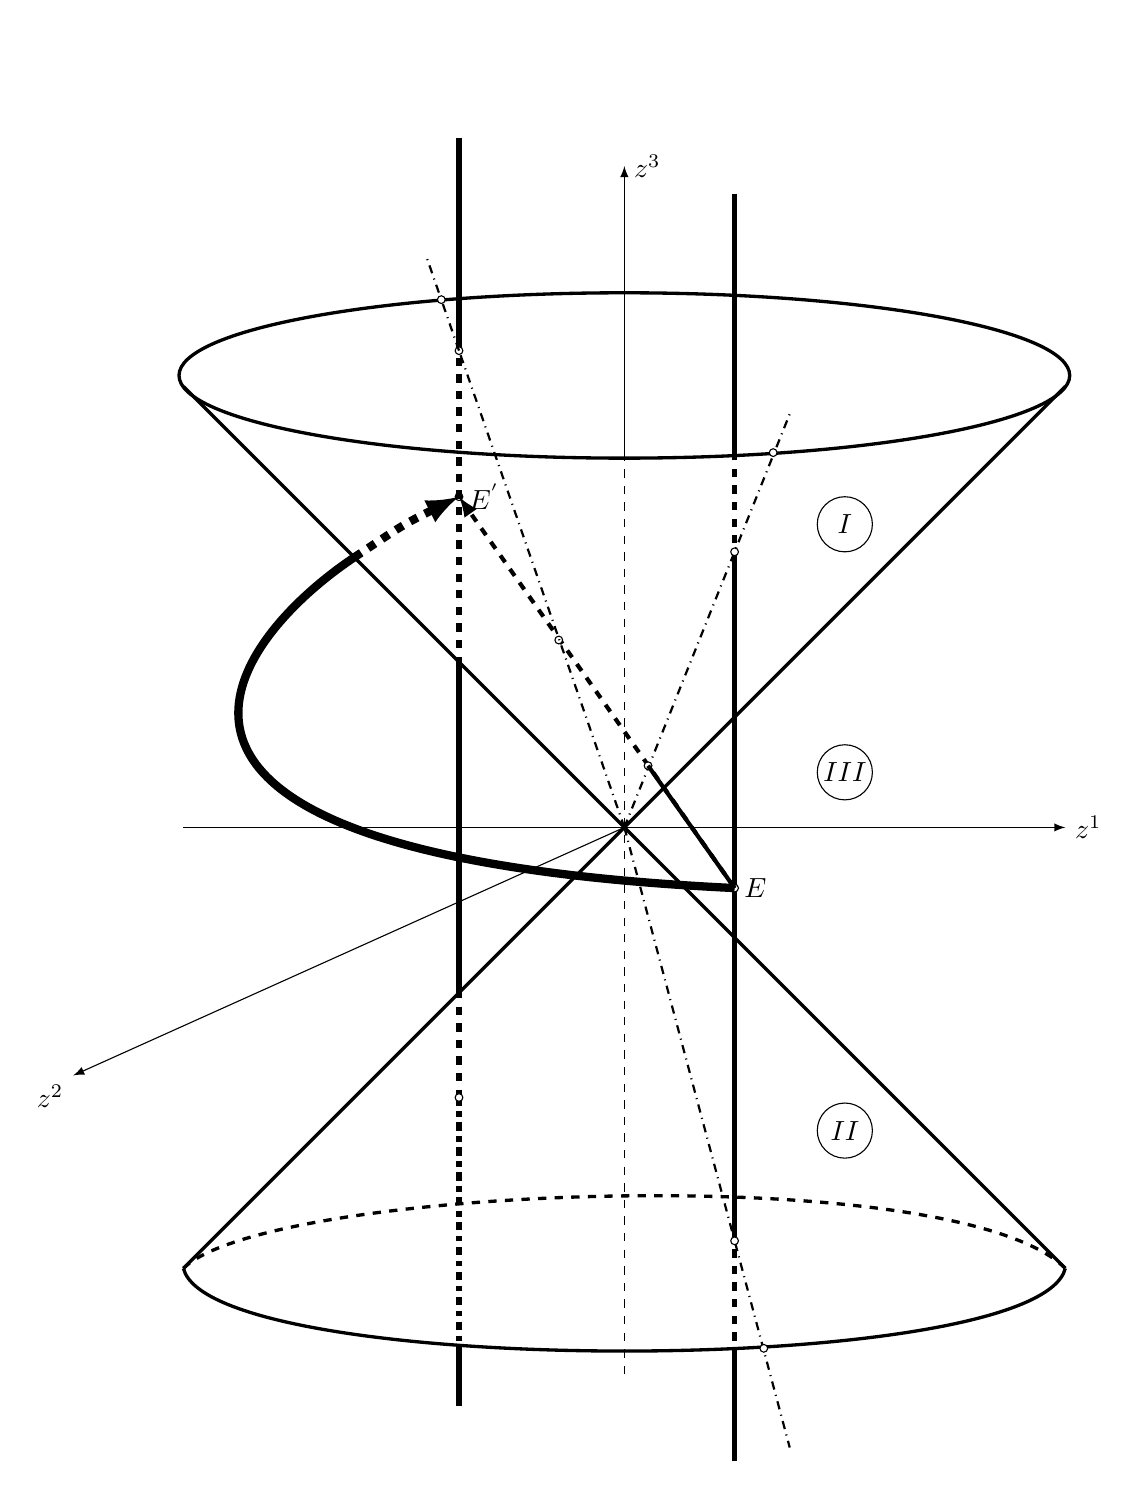
\begin{tikzpicture}[scale=0.70]
\coordinate (v1) at (-8,-0);
\coordinate (v2) at (8,-0) ;
\coordinate (v3) at (0,12) {};
\coordinate (v4) at (0,6.8) {};
\coordinate (v5) at (8,8) {};
\coordinate (v6)  at (0,0) {};
\coordinate (v7) at (-8,-8) {};
\coordinate (v8) at (8,-8) {};
\coordinate (v9) at (-8,8) {};
\coordinate (v10) at (-0,-10) {};
\coordinate (v11)  at (-10,-4.5) {};
\draw[-{latex}]  (v1)-- (v2)node[right] {$z^1$};
\draw  [-{latex}](v4)-- (v3)node[right] {$z^3$};
\draw  [-{latex}](v6)-- (v11)node[{anchor=north east}] {$z^2$};
\draw  [dashed](v4)-- (v10);
\draw[very thick]  (0,8.2) ellipse (8.08 and 1.5);
\draw [very thick] (v6) -- (v5);
\draw [very thick] (v7) -- (v6);
\draw  [very thick](v6) -- (v8);
\draw  [very thick](v6) -- (v9);
\draw[very thick] (-8,-8) .. controls (-7.5,-10) and (7.5,-10) .. (8,-8);
\draw [very thick, dashed,](-8,-8) .. controls (-6.5,-6.5) and (6,-6) .. (8,-8);

\coordinate (p0) at (-3.1,-1.4) {} {};
\coordinate (p1) at (2,-1.5) {} {};
\coordinate (p2) at (2,5) {} {};
\coordinate (p3) at (2,-7.5) {} {};
\coordinate (p4) at (5.5,0) {};

\draw [line width=2] (p2) -- (p1);
\draw [line width=2] (p2) -- (p3);
\coordinate (p5) at (2,6.7) {};
\coordinate (p6) at (2,-9.5) {};
\coordinate (p7)at (2,11.5) {};
\coordinate (p8)  at (2,-11.5) {};
\draw [dashed, line width=2] (p3) -- (p5);
\draw  [dashed, line width=2] (p2) -- (p6);
\draw [ line width=2] (p7) -- (p5);
\draw[ line width=2] (p8) -- (p6);

\coordinate (p9)  at (1.5*2,-1.5*7.5) {};
\coordinate (p10)  at (1.5*2,1.5*5) {};
\draw  [dashdotted,thick](v6) -- (p9);
\draw  [dashdotted,thick](v6) -- (p10);
\coordinate (t1) at (4,5.5) {};
\coordinate (t2) at (4,1) {} ;
\coordinate (t3) at (4,-5.5) {};
\draw[fill=black](t1)node[] {$I$};
\draw[fill=black](t2)node[] {$III$};
\draw[fill=black](t3)node[] {$II$};
\coordinate (t4) at (2.7,6.8) {};
\coordinate (t5) at (2.53,-9.45) {};
\draw[fill=white](t4) circle(2pt);
\draw[fill=white](t5) circle(2pt);

\draw  (t1) ellipse (0.5 and 0.5);
\draw  (t2) ellipse (0.5 and 0.5);
\draw  (t3) ellipse (0.5 and 0.5);
\draw  (-1.5,14.5) ellipse (0 and 0);
\coordinate (q1) at (2,-1.1) {} {} {};
\coordinate (q2) at (-3,6) {} {};
\draw[fill=white](q1) circle(2pt)node[{anchor=west }] {$E^{}$};
\draw[fill=white](q2) circle(2pt)node[{anchor=west }] {$E^{'}$};
\coordinate(q3) at (-4.9,4.9) {};
\draw [line width=3](q1) .. controls (-10.5,-0.5) and (-7,3.5) .. (q3);

\draw [line width=3,dashed, -latex](q3) .. controls (-4,5.5) and (-4,5.5) .. (q2);
\coordinate(s0) at (-3,12.5) {};
\coordinate(s1) at (-3,8.65) {};
\coordinate(s2) at (-3,-4.9) {};
\coordinate(s3) at (-3,2.95) {};
\coordinate(s4) at (-3,-2.95) {};
\coordinate(s5) at (-3,-9.5) {};
\coordinate(s6) at (-3,-10.5) {};
\coordinate(s7) at (-3*1.2,8.65*1.2) {};
\coordinate(s8) at (-3*1.107,8.65*1.107) {};
\draw [line width=2] (s1) -- (s0);
\draw [line width=2,dashed] (s3) -- (s1);
\draw [line width=2] (s3) -- (s4);
\draw [line width=2,dashdotted] (s2) -- (s5);
\draw [line width=2,dashed] (s4) -- (s2);
\draw [line width=2] (s5) -- (s6);
\draw[fill=white](s1) circle(2pt);
\draw[fill=white](s2) circle(2pt);
\draw[fill=white](p3) circle(2pt);
\draw[fill=white](p2) circle(2pt);
\draw [line width=1.5, dashed,-latex] (q1) -- (q2);
\coordinate(w0) at (-1*1.19,3.4) {} {};
\coordinate(w1)  at (0.43,1.12) {};
\draw[fill=white](w0) circle(2pt);
\draw[fill=white](w1) circle(2pt);
\draw  [dashdotted,thick](v6) -- (s1);
\draw  [dashdotted,thick](s1) -- (s7);
\draw[fill=white](s8) circle(2pt);
\draw [line width=1.5, ] (w1) -- (q1);
\end{tikzpicture}
\caption{Travelling between two points in region III (present) in a  $V_3$ space-time manifold}
\label{fig:fig_p96_3415_b}
\end{figure}
\end{comment}
$$\blacklozenge$$
\newpage

\section{p133 - Exercise}
\begin{tcolorbox}
In a space of two dimensions prove the relation
$$\mathbf{4.318.}\spatie \epsilon_{mp}\epsilon_{mq} = \delta_{pq}$$
\end{tcolorbox}
Suppose $p=q$, then in the summation the term is $0$ if $m=p=q$ and the remaining term is $1\times 1$ or $-1\times -1$ giving indeed $\delta_{pq}=1$.\\ 
If  $p\neq q$ we get either $m=p$ or $m=q$ in each term of the summation and hence all terms vanish.
$$\blacklozenge$$
\newpage

\section{p135 - Clarification}
\begin{tcolorbox}
$$\mathbf{4.324.}\spatie P_{mn}= \epsilon_{mnrs}X_rY_s$$
In 4.323 a skew-symmetric tensor is formed.
\end{tcolorbox}
Let's check whether $P_{mn}$ is indeed a tensor and if it is an oriented one.
Be an orthogonal transformation (proper or not)
\begin{align}
X^{'}_r = A_{rm}X_m+A_r
\end{align}
and let's check how the expression $P^{'}_{mn}= P_{rs}\partial_m X_r \partial_n X_s$ behaves.

\begin{align}
P^{'}_{mn}&= P_{rs}\partial_m z_r \partial_n z_s\\
\mathbf{(4.303.)\ }\Rightarrow \spatie &= \epsilon_{rspq}X_pY_q A_{mr}A_{ns}
\end{align}
From (4.302.) we have
\begin{align}
X_p = A_{kp}X^{'}_k -  A_{kp}A_k
\end{align}
Replacing this in (3)
\begin{align}
P^{'}_{mn}&=  \epsilon_{rspq}\left(A_{kp}X^{'}_k -  A_{kp}A_k\right)\left(A_{tq}Y^{'}_t -  A_{tq}A_t\right) A_{mr}A_{ns}\\
&=\left\{\begin{array}{l}
\epsilon_{rspq}A_{mr}A_{ns}A_{kp}A_{tq}X^{'}_kY^{'}_t \\\\
-\epsilon_{rspq}A_{mr}A_{ns}A_{kp}A_{tq}X^{'}_kA_t \\\\
-\epsilon_{rspq}A_{mr}A_{ns}A_{kp}A_{tq}Y^{'}_tA_k \\\\
+\epsilon_{rspq}A_{mr}A_{ns}A_{kp}A_{tq}A_kA_t 
\end{array}\right.\\
&= \epsilon_{rspq}A_{mr}A_{ns}A_{kp}A_{tq}\left(X^{'}_k-A_k\right)\left(Y^{'}_t-A_t\right)
\end{align}
A analogous reasoning as in (4.316.) gives us $\epsilon_{mnkt}\left|A_{mr}\right|=\epsilon_{rspq}A_{mr}A_{ns}A_{kp}A_{tq}$ and so 
\begin{align}
P^{'}_{mn}&= \epsilon_{mnkt}\left|A_{mr}\right| \left(X^{'}_k-A_k\right)\left(Y^{'}_t-A_t\right)
\end{align}
Apparently, even with $\left|A_{mr}\right| =1$ , $P_{mn}$ does not behave like a tensor due to the $ \left(X^{'}_k-A_k\right)\left(Y^{'}_t-A_t\right)$ components. But of course, this is consequence of the sloppy use of the transformation equation: equation (1) is the transformation rule for a point in the $V_4$ space but the object $P_{mn}$ takes two vectors as input. If we consider a vector as an object defined by an ordered pair i.e. $X\equiv \left(z^{(1)}_{(X)}, z^{(0)}_{(X)}\right)$ then $P_{mn}$ should be defined as $P_{mn}= \epsilon_{mnrs}\left(z^{(1)}_{(X)r}- z^{(0)}_{(X)r}\right)\left(z^{(1)}_{(Y)s}- z^{(0)}_{(Y)s}\right)$. This means that when using the transformation rule (1) we will get $$X^{'}\equiv \left(z^{'(1)}_{(X)}, z^{'(0)}_{(X)}\right)$$ giving as components 
\begin{align}X^{'}_r &= z^{'(1)}_{(X)r}- z^{'(0)}_{(X)r}\\&=   A_{rm}z^{(1)}_{(X)m}+A_r-A_{rm}z^{(0)}_{(X)m}-A_r\\
&= A_{rm}\left(z^{(1)}_{(X)m} -z^{(0)}_{(X)m}\right)
\end{align}
Replacing all this we get as a more correct representation of $p_{mn}$ and $P^{'}_{mn}$:
\begin{align}
\left\{\begin{array}{l}
P_{mn}= \epsilon_{mnrs}\left(z^{(1)}_{(X)r}- z^{(0)}_{(X)r}\right)\left(z^{(1)}_{(Y)s}- z^{(0)}_{(Y)s}\right)\\\\
P^{'}_{mn}= \epsilon_{mnkt}\left|A_{mr}\right| \left(z^{'(1)}_{(X)r}- z^{'(0)}_{(X)r}\right)\left(z^{'(1)}_{(Y)s}- z^{'(0)}_{(Y)s}\right)\\\\
\end{array}\right.
\end{align}
We see that indeed $P_{mn}$ is an oriented Cartesian tensor.
$$\blacklozenge$$
\newpage

\section{p135 - Exercise}
\begin{tcolorbox}
Write out the six independent non-zero components of $P_{mn}$ as given by $\mathbf{4.324.}$
\end{tcolorbox}
We have 
\begin{align}
\mathbf{4.324.}\spatie P_{mn}= \in_{mnrs}X^rY^s\\
\text{with}\quad \spatie m=n \quad \Rightarrow \quad P_{mn}= 0
\end{align}
So, the six independent components are in the set $\{mn\}= \left\{12,13,14,23,24,34 \right\}$ as $P_{nm}=-P_{mn}$.
\begin{align}
&\left\{\begin{array}{l}\\
P_{12} = \in_{1234}X^3Y^4+\in_{1243}X^4Y^3\\\\
P_{13} = \in_{1324}X^2Y^4+\in_{1342}X^4Y^2\\\\
P_{14} = \in_{1423}X^2Y^3+\in_{1432}X^3Y^2\\\\
P_{23} = \in_{2314}X^1Y^4+\in_{2341}X^4Y^1\\\\
P_{24} = \in_{2413}X^1Y^3+\in_{2431}X^3Y^1\\\\
P_{34} = \in_{3412}X^1Y^2+\in_{3421}X^2Y^1\\\\
\end{array}\right.\\
&\left\{\begin{array}{l}\\
P_{12} = X^3Y^4-X^4Y^3\\\\
P_{13} = -X^2Y^4+X^4Y^2\\\\
P_{14} = X^2Y^3-X^3Y^2\\\\
P_{23} = X^1Y^4-X^4Y^1\\\\
P_{24} = -X^1Y^3+X^3Y^1\\\\
P_{34} = X^1Y^2-X^2Y^1\\\\
\end{array}\right.
\end {align}
$$\blacklozenge$$
\newpage

\section{p136 - Exercise}
\begin{tcolorbox}
Translate the well-known vector relations
$$A\times (B\times C)= B(A.  C)-C(A.B)$$
$$\nabla \times (\nabla \times V)= \nabla (\nabla .  V )-\nabla^2V$$
into Cartesian tesnor form, and prove the by use of $4.329$.
\end{tcolorbox}
We have 
\begin{align}
\mathbf{4.329.}\spatie \in_{mrs}\in_{mpq} = \delta_{rp}\delta_{sq}-\delta_{rq}\delta_{sp}
\end{align}
The first identity
\begin{align}
A\times (B\times C)= B(A.  C)-C(A.B)\\
\Leftrightarrow\spatie \in_{npm}\in_{mrs}A_p B_r C_s = A_p\left(B_n C_p-C_n B_p\right)
\end{align}
Indeed,
\begin{align}
(B\times C)_m &= \in_{mrs}B_rC_s\\
\Rightarrow\spatie \left(A\times (B\times C)\right)_n &=\in_{npm}A_p \in_{mrs}B_rC_s\\
&=-\in_{mpn}\in_{mrs}A_p \in_{mrs}B_r C_s\\
&= -\delta_{pr}\delta_{ns}A_pB_rC_s+\delta_{ps}\delta_{nr}A_pB_rC_s\\
&= A_pB_nC_p-A_pB_pC_n\\
\Leftrightarrow\spatie & B(A.  C)-C(A.B)
\end{align}
The second identity
\begin{align}
\nabla \times (\nabla \times V)&= \nabla (\nabla .  V )-\nabla^2V\\
\Leftrightarrow \spatie \in_{nrm}\in_{mpq}V_{q,pr} &= V_{p,pn}- V_{n,pp}
\end{align}
Indeed,
\begin{align}
\left(\nabla \times V\right)_m &= \in_{mpq}V_{q,p}\\
\Rightarrow\spatie \left(\nabla  \times (\nabla \times V)\right)_n &=\in_{nrm}\left(\in_{mpq}V_{q,p}\right)_{,r}\\
 &=\in_{nrm}\in_{mpq}V_{q,pr}\\
 &=\delta_{rq}\delta_{np}V_{q,pr}-\delta_{pr}\delta_{nq}V_{q,pr}\\
 &= V_{p,pn}-V_{n,pp}
\end{align}
We have also
\begin{align}
\left(\nabla V\right) &= V_{p,p}\\
\Rightarrow\spatie \left(\nabla (\nabla .  V )\right)_n &= \left(V_{p,p}\right)_n\\
&= V_{p,pn}
\end{align}
and 
\begin{align}
\nabla^2 V_n  & \equiv  V_{n,pp} \\
\Rightarrow\spatie \left(\nabla (\nabla .  V )\right)_n- \nabla^2 V_n &= V_{p,pn}- V_{n,pp}
\end{align}
which corresponds to (15).
So the tensor expression in Cartesian tensor form can be written as 
$$\in_{nrm}\in_{mpq}V_{q,pr} = V_{p,pn}- V_{n,pp}$$

$$\blacklozenge$$
\newpage

\section{p139 - Exercise 1.}
\begin{tcolorbox}
Show that, in a 3-space of constant curvature $-\frac{1}{R^2}$ and positive definite metric form, the line element in polar coordinate is 
$$ds^2= dr^2+R^2\sinh^2\left(\frac{r}{R}\right)\left(d\theta^2+\sin^2\theta d\phi^2\right)$$
\end{tcolorbox}
We have by $4.120c$
\begin{align}
X_r \eta^r &= A\sinh \left(s\sqrt{-\epsilon K}\right)
\end{align}
We choose $N$ different $X^{(k)}_r$ $(k= 1,2,\dots, N)$ which are orthonormal.
Applying $(1)$ $N$ times with the different $X^{(k)}_r$ $(k= 1,2,\dots, N)$, we get
\begin{align}
X^{(k)}_r \eta^r &= A^{(k)}\sinh \left(s\sqrt{-\epsilon K}\right)
\end{align}
But as the $X^{(k)}_r$ are orthonormal and are used as a basis at the considered point of the geodesic we have 
\begin{align}
X^{(k)}_r &= \delta^k_r
\end{align}
So, $(2)$ becomes
\begin{align}
\eta^k &= A^{(k)}\sinh \left(s\sqrt{-\epsilon K}\right)
\end{align}
which are the components of the displacement vector in the orthonormal basis. By $\mathbf{2.301.}$ :
\begin{align}
Y^2 &= \epsilon a_{mn} Y^m Y^n\\
\Rightarrow \spatie \eta^2 &= \epsilon a_{mn} A^{(m)} A^{(n)}\sinh^2 \left(s\sqrt{-\epsilon K}\right)\\
\Rightarrow \spatie \eta &= C\left|\sinh \left(s\sqrt{-\epsilon K}\right)\right|\\
\text{with}\spatie C&= \sqrt{\left|\epsilon a_{mn} A^{(m)} A^{(n)}\right|}
\end{align}
As $\epsilon =1$ (positive-definite metric) and $K=-\frac{1}{R^2}$
we have
\begin{align}
\eta &= C\left|\sinh \left(\frac{s}{R}\right)\right|
\end{align}
From this and using the very same reasoning from $4.126.$ to $4.130.$ (pages 117-119) we get 
$$ds^2= dr^2+R^2\sinh^2\left(\frac{r}{R}\right)\left(d\theta^2+\sin^2\theta d\phi^2\right)$$
$$\blacklozenge$$
\newpage


\section{p139 - Exercise 2.}
\begin{tcolorbox}
Show that the volume of an antipodal 3-space of positive-definite metric form and positive constant curvature $\frac{1}{R^2}$ is $2\pi^2R^3$. (Use the equation 4.130. to find the area of a sphere $r= \text{constant}$ in polar coordinates. Multiply by $dr$ and integrate for $0\leq r \leq \pi R$ to get the volume). What is the volume if the space is polar?
\end{tcolorbox}
We have  $4.130$
\begin{align}
ds^2= dr^2+R^2\sin^2\left(\frac{r}{R}\right)\left(d\theta^2+\sin^2\theta d\phi^2\right)
\end{align}
Having a positive-definite metric form, the space can be locally considered as Euclidean and an elementary area of a  surface with constant $r (\rightarrow dr=0)$ can be calculated as $dS=ds_{d\theta=0}ds_{d\phi=0}$ and get by (1)
\begin{align}
dS &= R^2\sin^2\left(\frac{r}{R}\right)\sin\theta d\phi d\theta\\
\Rightarrow\spatie\frac{S}{8} &= R^2\sin^2\left(\frac{r}{R}\right)\int^{\frac{\pi}{2}}_{0}\int^{\frac{\pi}{2}}_{0} \sin\theta d\phi d\theta\\ 
&= R^2\sin^2\left(\frac{r}{R}\right)\frac{\pi}{2} \left.\left(-\cos\theta \right)\right|^{\frac{\pi}{2}}_{0}\\
\Rightarrow\spatie S&= 4\pi R^2\sin^2\left(\frac{r}{R}\right)
\end{align}
We see that the area is a cyclic function of $r$ having zeros' at $r= k\frac{\pi}{R }, k=1,2,\dots$
\begin{figure}[H]
\begin{center}
\begin{tikzpicture}[]
    \begin{axis}[
    domain = 0:2.5*pi,
    samples = 201,
    axis on top = true,
    grid =none,
    grid style = {dashed, line width=.1pt, draw=gray!30, 
    /pgfplots/on layer=axis background},
    		ytick=\empty,
		xtick=\empty,
		xmin=-0,
		xmax=9,
		ymin=0,
		ymax=1.5,
]
\addplot+[no marks, color=black] {(sin(deg(x)))^2};
\node[{anchor=south east}] at (0,10){$\phi_0$};
\end{axis}
\coordinate(0) at (0,0);
\node[{anchor=north east }] at (0){$0$};
\coordinate(p1) at (2.7,0);
\node[{anchor=north east }] at (p1){$\pi$};
\coordinate(p2) at (2*2.5,0);
\node[{anchor=north east }] at (p2){$2\pi$};
\end{tikzpicture}
\caption{Area of an antipodal 3-space of positive-definite metric form}
\label{fig:fig_p138_Ex2}
\end{center}
\end{figure}
So, there are good reasons to restrict $r$ to $[0,\pi R]$ as otherwise all space of that type would have infinite volume, whatever it's curvature. So, we get as volume 
\begin{align}
V &= 4\pi R^2\int^{\pi R}_{0}\sin^2\left(\frac{r}{R}\right)dr\\
&= 4\pi R^3\int^{\pi R}_0\sin^2\left(\frac{r}{R}\right)d\left(\frac{r}{R}\right)\\
&= 4\pi R^3\left.\left( \half x - \frac{1}{4}\sin2x \right)\right|^{\pi}_0\\
&= 2\pi^2 R^3
\end{align}
Fo a polar space, the volume would be half of that of an antipodal one (with same curvature of course) as in (3) we would consider only 4 quadrants instead of 8.
$$\blacklozenge$$
\newpage


\section{p139 - Exercise 3.}
\begin{tcolorbox}
By direct calculation of the tensor $R_{rsmn}$ verify that $\mathbf{4.130.}$ is the metric form of a space of constant curvature.
\end{tcolorbox}
We have  $4.130$
\begin{align}
ds^2&= dr^2+R^2\sin^2\left(\frac{r}{R}\right)\left(d\theta^2+\sin^2\theta d\phi^2\right)\\
\Rightarrow\spatie &
\ (a_{mn}) = \begin{pmatrix}
 1& 0 & 0\\
0 & R^2\sin^2\left(\frac{r}{R}\right) & 0 \\
0 & 0 & R^2\sin^2\left(\frac{r}{R}\right)\sin^2\theta \\
\end{pmatrix}
\end{align}
Now for $R_{rsmn}$ we refer to exercise 7 page 109 of chapter 3, where the curvature tensor was calculated for a general case of the form 
$$ ds^2= (h_1dx^1)^2+(h_2dx^2)^2+(h_3dx^3)^2$$ where $h_1, h_2, h_3$ are functions of the three coordinates.
We have then for our case
\begin{align}
\left\{\begin{array}{l}
h_1 = 1\\\\
h_2 = R\sin\left(\frac{r}{R}\right)\\\\
h_3 = R\sin\left(\frac{r}{R}\right)\sin\theta\\\\
\end{array}\right.
\end{align}
In the exercise we got for the non-vanishing curvature tensors
\begin{align}
R_{1212}&=
-h_2\partial_{11}^2(h_2)-h_1\partial_{22}^2(h_1)
+\frac{h_2}{h_1}\partial_1 h_1\partial_1 h_2+\frac{h_1}{h_2}\partial_2 h_1\partial_2 h_2-\frac{h_1 h_2}{h_3^2}\partial_3 h_1\partial_3 h_2\\
R_{2323}&=
-h_3\partial_{22}^2(h_3)-h_2\partial_{33}^2(h_2)
+\frac{h_3}{h_2}\partial_2 h_2\partial_2 h_3+\frac{h_2}{h_3}\partial_3 h_2\partial_3 h_3-\frac{h_2 h_3}{h_1^2}\partial_1 h_2\partial_1 h_3\\
R_{1313}&=
-h_3\partial_{11}^2(h_3)-h_1\partial_{33}^2(h_1)
+\frac{h_3}{h_1}\partial_1 h_1\partial_1 h_3+\frac{h_1}{h_3}\partial_3 h_1\partial_3 h_3-\frac{h_1 h_3}{h_2^2}\partial_2 h_1\partial_2 h_3
\end{align}
\begin{align}
R_{1213}&=-h_1\partial_{32}^2(h_1)+\frac{h_1}{h_3}\partial_2 h_3\partial_3 h_1+\frac{h_1}{h_2}\partial_2 h_1\partial_3 h_2\\
R_{1223}&=h_2\partial_{31}^2(h_2)-\frac{h_2}{h_1}\partial_1 h_2\partial_3 h_1-\frac{h_2}{h_3}\partial_3 h_2\partial_1 h_3\\
R_{1323}&=
-h_3\partial_{21}^2(h_3)+\frac{h_3}{h_1}\partial_1 h_3\partial_3 h_1+\frac{h_3}{h_2}\partial_2 h_3\partial_1 h_2
\end{align}
Clearly $\partial_{k}^2(h_1)=0$ and $\partial_{mn}^2(h_1)=0$ and considering $h_2 = h_2(r), \ h_3 = h_3(r,\theta)$
we can simplify 
\begin{align}
R_{1212}&=
-h_2\partial_{11}^2(h_2)\\
R_{2323}&=
-h_3\partial_{22}^2(h_3)
-\frac{h_2 h_3}{h_1^2}\partial_1 h_2\partial_1 h_3\\
R_{1313}&=
-h_3\partial_{11}^2(h_3)
\end{align}
\begin{align}
R_{1213}&=0\\
R_{1223}&=0\\
R_{1323}&=
-h_3\partial_{21}^2(h_3)+\frac{h_3}{h_2}\partial_2 h_3\partial_1 h_2
\end{align}
with 
\begin{align}
\left\{\begin{array}{l}
\partial_1 h_2=\cos\left(\frac{r}{R}\right)\\\\
\partial_1 h_3=\cos\left(\frac{r}{R}\right)\sin\theta\\\\
\partial_2 h_3=R\sin\left(\frac{r}{R}\right)\cos\theta\\\\
\partial^2_{11} h_2=-\frac{1}{R}\sin\left(\frac{r}{R}\right)\\\\
\partial^2_{11} h_3=-\frac{1}{R}\sin\left(\frac{r}{R}\right)\sin\theta\\\\
\partial^2_{21} h_3=\cos\left(\frac{r}{R}\right)\cos\theta\\\\
\partial^2_{22} h_3=-R\sin\left(\frac{r}{R}\right)\sin\theta\\\\
\end{array}\right.
\end{align}
giving
\begin{align}
R_{1212}&=
\sin^2\left(\frac{r}{R}\right)\\
R_{2323}&=
R^2\sin^2\left(\frac{r}{R}\right)\sin^2\theta 
-R^2\sin^2\left(\frac{r}{R}\right)\sin^2\theta\cos^2\left(\frac{r}{R}\right)\\
&= R^2\sin^4\left(\frac{r}{R}\right)\sin^2\theta\\
R_{1313}&=\sin^2\left(\frac{r}{R}\right)\sin^2\theta\\
R_{1213}&=0\\
R_{1223}&=0\\
R_{1323}&=
-R\sin\left(\frac{r}{R}\right)\sin\theta\cos\left(\frac{r}{R}\right)\cos\theta+\sin\theta R\sin\left(\frac{r}{R}\right)\cos\theta\cos\left(\frac{r}{R}\right)\\&=0
\end{align}
and considering the symmetries
\begin{align}
R_{1212}&=-R_{1221}=-R_{2112}=
\sin^2\left(\frac{r}{R}\right)\\
R_{2323}&=-R_{2332}=-R_{3223}= R^2\sin^4\left(\frac{r}{R}\right)\sin^2\theta\\
R_{1313}&=-R_{1331}=-R_{3113}=\sin^2\left(\frac{r}{R}\right)\sin^2\theta\\
\end{align}
By $\mathbf{4.114.}$
\begin{align}
R_{rsmn}&= K\left(a_{rm}a_{sn}-a_{rn}a_{sm}\right)\\
\Rightarrow\spatie &\left\{\begin{array}{l}
R_{1212}= K\left(a_{11}a_{22}-a_{12}a_{21}\right)\\
R_{2323}= K\left(a_{22}a_{33}-a_{23}a_{32}\right)\\
R_{1313}= K\left(a_{11}a_{33}-a_{13}a_{31}\right)
\end{array}\right.\\
\Rightarrow\spatie &\left\{\begin{array}{l}
R_{1212}= K R^2\sin^2\left(\frac{r}{R}\right)\\
R_{2323}= K R^2\sin^2\left(\frac{r}{R}\right)R^2\sin^2\left(\frac{r}{R}\right)\sin^2\theta\\
R_{1313}= K R^2\sin^2\left(\frac{r}{R}\right)\sin^2\theta\\
\end{array}\right.\\
\Rightarrow\spatie &\left\{\begin{array}{l}
R_{1212}= K R^2\sin^2\left(\frac{r}{R}\right)\\
R_{2323}= K R^4\sin^4\left(\frac{r}{R}\right)\sin^2\theta\\
R_{1313}= K R^2\sin^2\left(\frac{r}{R}\right)\sin^2\theta\\
\end{array}\right.
\end{align}
 replacing (25), (26) and (27) in (32) we get
 \begin{align}
\left\{\begin{array}{l}
\sin^2\left(\frac{r}{R}\right)= K R^2\sin^2\left(\frac{r}{R}\right)\\
R^2\sin^4\left(\frac{r}{R}\right)\sin^2\theta= K R^4\sin^4\left(\frac{r}{R}\right)\sin^2\theta\\
\sin^2\left(\frac{r}{R}\right)\sin^2\theta= K R^2\sin^2\left(\frac{r}{R}\right)\sin^2\theta\\
\end{array}\right.
\end{align}
giving indeed for the three curvature tensors $K=\frac{1}{R^2}$\\
With this, the question of the  exercise is answered but we go a little bit further and investigate for this practical case the equations of $\mathbf{4.115.}$ and  calculate $R=a^{mn}R_{mn}$. With $R$, the curvature invariant. To avoid confusion with the curvature $R$ itself we use $\mathfrak{R}$ for the curvature invariant.\\
As the metric tensor is diagonal:

\begin{align}
\mathfrak{R}=a^{11}R_{11}+a^{22}R_{22}+a^{33}R_{33}\\
\end{align}
and 
\begin{align}
R_{mn}&= a^{sn}R_{srmn}\\
\Rightarrow\spatie &
\left\{\begin{array}{l}
R_{11} = a^{11}R_{1111}+a^{22}R_{2112}+a^{33}R_{3113}\\\\
R_{22} = a^{11}R_{1221}+a^{22}R_{2222}+a^{33}R_{3223}\\\\
R_{33} = a^{11}R_{1331}+a^{22}R_{2332}+a^{33}R_{3333}\\\\
\end{array}\right.\\
\Rightarrow\spatie &\left\{\begin{array}{l}
R_{11} = -a^{22}\sin^2\left(\frac{r}{R}\right)-a^{33}\sin^2\left(\frac{r}{R}\right)\sin^2\theta\\\\
R_{22} = -a^{11}\sin^2\left(\frac{r}{R}\right)-a^{33}R^2\sin^4\left(\frac{r}{R}\right)\sin^2\theta\\\\
R_{33} = -a^{11}\sin^2\left(\frac{r}{R}\right)\sin^2\theta-a^{22}R^2\sin^4\left(\frac{r}{R}\right)\sin^2\theta\\\\
\end{array}\right.\\
\Rightarrow\spatie &\left\{\begin{array}{l}
R_{11} = -\frac{\sin^2\left(\frac{r}{R}\right)}{R^2\sin^2\left(\frac{r}{R}\right)}-\frac{\sin^2\left(\frac{r}{R}\right)\sin^2\theta}{R^2\sin^2\left(\frac{r}{R}\right)\sin^2\theta}\\\\
R_{22} = -\sin^2\left(\frac{r}{R}\right)-\frac{R^2\sin^4\left(\frac{r}{R}\right)\sin^2\theta}{R^2\sin^2\left(\frac{r}{R}\right)\sin^2\theta}\\\\
R_{33} = -\sin^2\left(\frac{r}{R}\right)\sin^2\theta-\frac{R^2\sin^4\left(\frac{r}{R}\right)\sin^2\theta}{R^2\sin^2\left(\frac{r}{R}\right)}\\\\
\end{array}\right.
\end{align}
giving
\begin{align}
\left\{\begin{array}{l}
R_{11} = -\frac{2}{R^2}\\\\
R_{22} = -2\sin^2\left(\frac{r}{R}\right)\\\\
R_{33} = -2\sin^2\left(\frac{r}{R}\right)\sin^2\theta\\\\
\end{array}\right.
\end{align}
hence
\begin{align}
\mathfrak{R}&=a^{11}R_{11}+a^{22}R_{22}+a^{33}R_{33}\\
\Rightarrow\spatie \mathfrak{R}&= -\frac{2}{R^2}-2\frac{\sin^2\left(\frac{r}{R}\right)}{R^2\sin^2\left(\frac{r}{R}\right)}-2\frac{\sin^2\left(\frac{r}{R}\right)\sin^2\theta}{R^2\sin^2\left(\frac{r}{R}\right)\sin^2\theta }\\
&= -\frac{6}{R^2}
\end{align}
The equations in (40) and (43) are indeed in accordance with $\mathbf{4.115}$ .
$$\blacklozenge$$
\newpage

\section{p139 - Exercise 4}
\begin{tcolorbox}
Show that if $V_N$ has positive-definite metric form and constant positive curvature $K$, then coordinates $y^r$ exist so that
$$ds^2=\frac{dy^m dy^m}{\left(1+\kwart y^n y^n\right)^2}$$
(Starting with a coordinate system $x^r$ which is locally Cartesian at $O$, take at any point $P$ the coordinates
$$y^r=p^r\frac{2}{\sqrt{K}}\tan\left(\half r \sqrt{K}\right)$$
where $p^r$ ar the the components of the unit tangent vector $\left(\dv{x^r}{s}\right)$ at $O$ to the geodesic $OP$ and $r$ is the geodesic distance $OP$.)
\end{tcolorbox}
Let us first understand what happens. Fig.1.5 for a $V_3$ will help us understand.
Let $P$ and $P+dP$ be two points separated by an infinitesimal distance. Consider the two geodesics initiated from the origin and joining these two points. Be $X$ and $X^{'}$ the two tangents unit vectors  to these geodesics. Those vectors have components $p^r=\dv{x^r}{s}$ taken along their respective geodesics.  By the considered transformation the points $P$ and $P+dP$ are mapped on the  points  $\tau (P)$ and $\tau (P+dP)$ with $\left|O\tau (P)\right|$ and $\left|O\tau (P+dP)\right|$ collinear with the  two tangents unit vectors  $X$ and $X^{'}$ . \\
Observe also the segment $PN$ which corresponds to the geodesic displacement $\eta$ for the geodesic distance $r=OP$. As the metric form is positive-definite, we can consider that the infinitesimal triangle $\left|\widehat{PNP+dP}\right|$ lies in an infinitesimally Euclidean space and  we can express $ds^2=\eta^2+ dr^2$ as $\left|NP+dP\right| = dr$. Observe now, the triangle $\left|\widehat{\tau(P)\tau(N)\tau(P+dP)}\right|$. There also we have $\left|\tau(P+dP)\tau(P)\right|^2 = \left|\tau(P)\tau(N)\right|^2+\left|\tau(P+dP)\tau(N)\right|^2$. Can we find a relationship between these two triangle?\\
\begin{figure}[H]
\begin{center}
\usetikzlibrary {arrows.meta}
\begin{tikzpicture}

\coordinate (v1) at (-0.5,0) {};
\coordinate  (v2) at (-0.5,10.5) {} {};
\coordinate  (v4) at (-5,-3.5) {};
\coordinate  (v3) at (11,0) {};
\draw [-{Latex[length=3mm]}] (v1) -- (v2);
\draw  [-{Latex[length=3mm]}] (v1)-- (v3);
\draw   [-{Latex[length=3mm]}](v1) -- (v4);

\coordinate  (c1) at (7,2) {};
\coordinate  (c2) at (8,4.5) {};
\draw[ultra thick]  plot[,smooth, tension=.7] coordinates {(v1) (3.5,1.4) (c1)};
\draw [ultra thick]  plot[smooth, tension=.7] coordinates {(v1) (1.5,2.5) (c2)};

\coordinate  (v5) at (1,3.5) {};
\coordinate  (v5b) at (2*1.25,2*3.5) {};
\draw  [dotted, very thick](v5) -- (v5b);
\coordinate  (v6) at (3,2) {};
\coordinate  (v6b) at (1.5*3.28,1.5*2) {};
\draw  [dotted, very thick](v6) -- (v6b);
\draw  [-{Latex[length=3mm]},thick](v1) -- (v6);
\draw [-{Latex[length=3mm]}, thick] (v1) -- (v5);
\draw[thin,dashdotted,-{Latex[length=3mm]}]   plot[smooth, tension=.7] coordinates {(c2) (6.5,8) (v5b)};
\draw[thin,dashdotted,-{Latex[length=3mm]}]  plot[smooth, tension=.7] coordinates {(c1) (6.2,3.5) (v6b)};
\coordinate (v8) at (2.5,-1.5) {};
\coordinate (v7) at (-2.4,-1.5) {};
\coordinate (v9) at (4.5,0) {};
\coordinate (v10)at  (-0.5,8.5) {};
\draw  [dashed](v7) -- (v8);
\draw  [dashed](v5b)-- (v8);
\draw  [dashed](v5b)-- (v10);
\draw  [dashed](v8)-- (v9);
\draw  [dashed](v1)-- (v8);

\coordinate (w1) at (5,-2) {};
\coordinate (w2) at (7.5,0) {} {};
\coordinate (w3) at (-3.1,-2) {};
\coordinate (w4) at (-0.5,5.5) {};
\draw  [dashed](w1) -- (v6b);
\draw  [dashed](w1)-- (w2);
\draw  [dashed](w1)-- (w3);
\draw  [dashed](v6b)-- (w4);
\draw  [dashed](v1)-- (w1);

\draw[fill] (c1) circle (3pt);
\draw[fill] (c2) circle (3pt);
\draw[fill] (v5b) circle (3pt);
\draw[fill] (v6b) circle (3pt);

\draw[fill] (v7) circle (2pt);

\draw[fill] (v8) circle (2pt);
\draw[fill] (v9) circle (2pt);
\draw[fill] (v10) circle (2pt);

\draw[fill] (w1) circle (2pt);
\draw[fill] (w2) circle (2pt);
\draw[fill] (w3) circle (2pt);
\draw[fill] (w4) circle (2pt);

\node[label= east:$P$] at (c1) {};
\node[label=north east:$P+dP$] at (c2) {};
\node[label= east:$\tau(P+dP)$] at (v5b) {};
\node[label= east:$\tau(P)$] at (v6b) {};

\node[label=north west:$\tau(P)^2$] at (w2) {};
\node[label= west:$\tau(P)^1$] at (w3) {};
\node[label=west:$\tau(P)^3$] at (w4) {};


\node[label=north west :$\tau(P+dP)^2$] at (v9) {};
\node[label=west:$\tau(P+dP)^3$] at (v10) {};
\node[label=west:$\tau(P+dP)^1$] at (v7) {};
\node[label=west:$X^{'}$] at (v5) {};
\node[label=north :$X^{}$] at (v6) {};
\node[label=west :$O$] at (v1) {};


\coordinate (q1) at (6.5,4.15) {};
\draw[fill] (q1) circle (2pt);
\node[label=north  :$N$] at (q1) {};
\draw  [dashed,thick,red](c1)-- (q1);
\draw  [dashed,thick,red](c1)-- (c2);

\coordinate (q2) at (1.4*1.25,1.5*3.5) {};
\draw[fill] (q2) circle (2pt);
\node[label=north west :$\tau(N)$] at (q2) {};
\draw  [dashed,thick,red](v6b)-- (q2);

\draw  [dashed,thick,red](v6b)-- (v5b);
\draw[thin,dashdotted,-{Latex[length=3mm]}]  plot[smooth, tension=.7] coordinates {(q1) (4.2,6) (q2)};
 \draw[-Latex,red] let
    \p0 = (v1),
    \p1 = (v6),
    \p2 = (v5),
    \n1 = {atan2(\y1 - \y0,\x1 - \x0)},
    \n2 = {atan2(\y2 - \y0,\x2 - \x0)},
    \n3 = {1cm},
    \n4 = {(\n1 + \n2) / 2}
  in (v1) +(\n1:\n3) arc[radius = \n3, start angle = \n1, end angle = \n2] node [midway,above right]{$\chi$};
\end{tikzpicture}
\caption{Coordinate system in constant curvature space}
\label{fig:fig_p139_Ex4}
\end{center}
\end{figure}

Let's define $\alpha (r) = \frac{2}{\sqrt{K}}\tan\left(\half r \sqrt{K}\right)$ so that $y^k = \alpha (r)p^k$
We have 
\begin{align}
\left\{\begin{array}{l}
\left|OX^{'}\right|= \left|OX^{}\right|=1\\\\
\left|O\tau (N)\right|= \left|O\tau (P)\right|=\alpha (r)\\\\
 \left|O\tau (P+dP)\right|=\alpha (r+dr)\\\\
\end{array}
\right.
\end{align}
Expanding the last equation in a Taylor series we get as first order term
\begin{align}
\left|\tau (N)\tau (P+dP)\right|= \frac{1}{\cos^2(\half r \sqrt{K})}dr
\end{align}
Also,
\begin{align}
\left|\tau (N)\tau (P)\right|= 2\alpha (r)\sin \frac{\chi}{2}  \approx \alpha (r) \chi 
\end{align}
From $\mathbf{4.124}$ we have $\chi=\left(\dv{\eta}{r}\right)_{r=0}= C\sqrt{K}$  .
But note also that from $\mathbf{4.122}$ we have for the geodesic displacement $\eta = C\left|\sin r\sqrt{K}\right|$. 
\begin{align}
C&= \frac{\eta }{\left|\sin r\sqrt{K}\right|}\\
\Rightarrow \spatie \chi&=\frac{\eta }{\left|\sin r\sqrt{K}\right|}\sqrt{K}\\
\Rightarrow \spatie \left|\tau (N)\tau (P)\right|&=\eta\frac{\sqrt{K} }{\left|\sin r\sqrt{K}\right|}\alpha (r) 
\end{align}
Let's put $\left|\tau (N)\tau (P)\right|=\hat{\eta}$.
\begin{align}
\hat{\eta}&=\eta\frac{\sqrt{K} }{\left|\sin r\sqrt{K}\right|}\alpha (r) 
\end{align}
At the point $P$ we have $\left|PN\right| = \eta$ and so
\begin{align}
ds^2=\eta^2+ dr^2
\end{align}
Let's put $\left|\tau(P+dP)\tau(P)\right|^2=d\hat{s}^2$.
\begin{align}
d\hat{s}^2 &= \hat{\eta}^2+\left|\tau(P+dP)\tau(N)\right|^2\\
\text{(2) and (7) }\Rightarrow\spatie &= \eta^2\frac{K }{\sin^2 (r\sqrt{K})}\frac{4}{K}\frac{\sin^2 (\half r \sqrt{K})}{\cos^2 (\half r \sqrt{K})}+ \frac{1}{\cos^4(\half r \sqrt{K})}dr^2\\
\sin r\sqrt{K} &= 2\sin (\half r\sqrt{K})\cos (\half r\sqrt{K})\\
\Rightarrow\spatie  d\hat{s}^2 &= \eta^2\frac{1}{\cos^4 (\half r \sqrt{K})}+ \frac{1}{\cos^4(\half r \sqrt{K})}dr^2\\
\Rightarrow\spatie \eta^2+dr^2 &= d \hat{s}^2 \cos^4(\half r \sqrt{K})\\
\Rightarrow\spatie ds^2 &= d \hat{s}^2 \cos^4(\half r \sqrt{K})
\end{align}
It is easy to see that $d \hat{s}^2 =  dy^k dy^k$ and also
\begin{align}
\cos^4(\half r \sqrt{K}) &= \left(\cos^2(\half r \sqrt{K})\right)^2\\
 &= \left(\frac{\cos^2(\half r \sqrt{K})}{\cos^2(\half r \sqrt{K})+\sin^2(\half r  \sqrt{K})}\right)^2\\
&= \left(\frac{1}{1+\tan^2(\half r  \sqrt{K})}\right)^2
\end{align}
We note that $\frac{2}{\sqrt{K}}\tan(\half r  \sqrt{K})$ is the size of the vector $\left|O\tau(P)\right|$ and can express this as (as we use local Cartesian coordinates at the origin) $\left|O\tau(P)\right|^2 = y^ky^k$ and thus $\tan^2(\half r  \sqrt{K}) =\frac{K}{4}y^ky^k$. Combining this with (14) and (17) gives:
\begin{align}
ds^2 &= d \hat{s}^2\left(\frac{1}{1+\frac{K}{4}y^ky^k}\right)^2
\end{align} 
which gives as final expression 
\begin{align}
ds^2 &= \frac{dy^k dy^k}{\left(1+\frac{K}{4}y^ky^k\right)^2}
\end{align}
$$\blacklozenge$$
\newpage

\section{p140 - Exercise 5}
\begin{tcolorbox}
Show that in a flat $V_n$ the straight line joining any two points of a $P$-flat $(P>N)$ lies entirely in the P-flat.
\end{tcolorbox}
For a $P$-flat we have by an appropriate re indexing of the variables $z_k$
\begin{align}
A_{mp}z_p+B_p =0 \spatie m=1,\dots,P
\end{align}
A straight line has as equation $z_p=C_p u + D_p$. As we have two points in the $P$-flat we have two $u_1, u_2$ for which yields
\begin{align}
&\left\{ \begin{array}{ll}
A_{mp}\left(C_p u_1 + D_p\right) +B_p =0&\\
 & \spatie m=1,\dots,P\\
A_{mp}\left(C_p u_2 + D_p\right) +B_p =0& 
\end{array}\right.
\end{align} 
Subtracting the corresponding equations in $m$ for the two sets $u_1, u_2$ gives 
\begin{align}
&A_{mp}C_p\left( u_1-u_0 \right) =0&\\
\Rightarrow\spatie &A_{mp}C_p=0\spatie &\text{ for }m=1,\dots,P\\
\text{(4) in (2) }\Rightarrow\spatie &A_{mp}D_p +B_p =0 \spatie &\text{ for }m=1,\dots,P
\end{align} 
So for an arbitrary $u$ we get from (1),(4) and (5)
\begin{align}
A_{mp}\left(C_p u + D_p\right) +B_p = \underbrace{A_{mp}C_p}_{=0} u + \underbrace{A_{mp}D_p +B_p}_{=0} \spatie &\text{ for }m=1,\dots,P
\end{align}
\begin{align}
\Rightarrow\spatie A_{mp}\left(\underbrace{C_p u + D_p}_{z_p}\right) +B_p =0 \spatie &\text{ for }m=1,\dots,P
\end{align}
So the points $z_p$ lying on the line satisfy the conditions for the  $P$-flat and lie therefore in the  $P$-flat.
$$\blacklozenge$$
\newpage

\section{p140 - Exercise 6}
\begin{tcolorbox}
Show that in four dimensions the transformation$$\begin{array}{l}
z^{'}_1 = z_1\cosh \phi + i z_4\sinh \phi\\
z^{'}_2 = z_2\\
z^{'}_3 = z_3\\
z^{'}_4 = -iz_1\sinh \phi +  z_4\cosh \phi
\end{array}$$
is orthogonal, $\phi$ being any constant. Putting $z_1=x,\ z_2 =y, \ z_3 = z, \ z_4 = ict, \ \phi = \frac{v}{c}$, obtain the transformation connecting $(x^{'},y^{'},z^{'},t^{'})$ and $(x^{},y^{},z^{},t^{})$. This is the $\mathit{Lorentz \ transformation} $ of the special theory of relativity.
\end{tcolorbox}
We can represent the transformation with the matrix
\begin{align}
\left(A_{mn}\right) &=
\begin{pmatrix}
 \cosh \phi&  0& 0 & i \sinh \phi \\
 0& 1 & 0 &0  \\
 0& 0 &  1&  0\\
 -i\sinh \phi&  0& 0 &  \cosh \phi \\
\end{pmatrix}
\end{align}
We use $\mathbf{4.210.}$ i.e. $A_{pm}A_{qm} = \delta _{pq}$ as a condition for the orthogonality of a transformation. This can be written in matrix form
\begin{align}
\left(A_{mn}\right)\left(A_{mn}\right)^{T}= \mathbf{I}
\end{align}
and get

\begin{align}
\left(A_{mn}\right)\left(A_{mn}\right)^{T}&=
\begin{pmatrix}
 \cosh \phi&  0& 0 & i \sinh \phi \\
 0& 1 & 0 &0  \\
 0& 0 &  1&  0\\
 -i\sinh \phi&  0& 0 &  \cosh \phi \\
\end{pmatrix}\begin{pmatrix}
 \cosh \phi&  0& 0 & -i \sinh \phi \\
 0& 1 & 0 &0  \\
 0& 0 &  1&  0\\
 i\sinh \phi&  0& 0 &  \cosh \phi \\
\end{pmatrix}\\
&= \begin{pmatrix}
 \cosh^2 \phi- \sinh ^2\phi &  0& 0 & -i \cosh \phi\sinh \phi +i \cosh \phi\sinh \phi  \\
 0& 1 & 0 &0  \\
 0& 0 &  1&  0\\
 i \cosh \phi\sinh \phi -i \cosh \phi\sinh \phi  &  0& 0 &  -\sinh^2 \phi + \cosh^2 \phi \\
\end{pmatrix}\\
&= \mathbf{I}
\end{align}
We now calculate the Lorentz transformation.\\
First note that 
\begin{align}
&\left \{\begin{array}{l}
\cosh y = \frac{e^y+e^{-y}}{2}\\
\sinh y = \frac{e^y-e^{-y}}{2}\\
\tanh^{-1}  x = \half \log \left(\frac{1+x}{1-x}\right)\\
\end{array}\right.\\
\Rightarrow\spatie  &\left \{ \begin{array}{l}
\cosh\left(\tanh^{-1}  x \right) = \frac{1}{\sqrt{1-x^2}}\\
\sinh\left(\tanh^{-1}  x \right) = \frac{x}{\sqrt{1-x^2}}
\end{array}\right.
\end{align}
Replacing $x$ with $\tanh \phi = \frac{v}{c}$ gives
\begin{align}
\left \{ \begin{array}{l}
\cosh \phi = \frac{1}{\sqrt{1-\frac{v^2}{c^2}}}\\
\sinh \phi = \frac{v}{c\sqrt{1-\frac{v^2}{c^2}}}
\end{array}\right.
\end{align}
and the transformation becomes
$$\begin{array}{l}
x^{'} = \frac{x- vt}{\sqrt{1-\frac{v^2}{c^2}}}\\
y{'} = y\\
z^{'} = z\\
t^{'} = \frac{t-\frac{vx}{c^2}}{\sqrt{1-\frac{v^2}{c^2}}} 
\end{array}$$
$$\blacklozenge$$
\newpage


\section{p140 - Exercise 7}
\begin{tcolorbox}
Prove that in a flat space a plane, defined by $\mathbf{4.22}$, is itself a flat space f $N-1$ dimensions.
\end{tcolorbox}
For a $N-1$-flat we have $\mathbf{4.22}$
\begin{align}
A^{'}_r z_r+B^{'}=0
\end{align}
Suppose that $A_N \ne 0$ then we can express $Z_N$, by dividing the equation $(1)$ by $A_N$ as 
\begin{align}
z_N = A_{\gamma} z_{\gamma}+B \spatie \text{ with } \gamma = 1,2, \dots, N-1
\end{align}
Then $\phi = z_nz_n$ becomes
\begin{align}
\phi &= d z_{\gamma}dz_{\gamma}+ dz_N dz_N\\
&=d z_{\gamma}dz_{\gamma} + \left(A_{\gamma} dz_{\gamma}\right)\left(A_{\tau} dz_{\tau}\right)\\
&=d z_{\gamma}dz_{\gamma} + A_{\gamma \tau} dz_{\gamma} dz_{\tau}
\end{align}
So $\phi$ can be expressed as $\phi = a_{\gamma \tau}dz_{\gamma}dz_{\tau}$.\\
But as $a_{\gamma \tau}$ are constants, the Christoffel symbols vanish and so does the curvature tensor $R^{\alpha}_{\beta \gamma \delta}$ in the $N-1$ space. Hence, the $V_{N-1}$ space delimited by equation (1) is flat.\\
Question: can we find the right orthogonal transformation so that the metric form in (5) can be made homogeneous?\\
The metric form in (5) can be represented as
\begin{align}
\left(a_{mn}\right) &= \begin{pmatrix}
 1-A_1^2& \half A_1A_{2} & \dots &  \half A_1A_{N-1}\\
 \half A_1A_{2}&  1-A_2^2&  \dots& \half A_2A_{N-1}\\
 \vdots& \vdots &  \ddots& \vdots\\
 \half A_1A_{N-1}&\half A_2A_{N-1}  & \dots & 1-A_{N-1}^2 \\
\end{pmatrix}
\end{align}

$$\blacklozenge$$
\newpage

\section{p140 - Exercise 8}
\begin{tcolorbox}
Show that in a flat space of positive-definite metric form, a sphere of zero radius consists of a single point, but that if the metric form is indefinite, a sphere of zero radius extends to infinity.
\end{tcolorbox}
A sphere is determined by $ z_kz_k= \pm R^2$ with $+$ for a positive definite metric and $\pm$ if the metric is indefinite.\\
For a positive definite metric a zero radius sphere has the equation $ z_n z_n= 0$. It is obvious that as $z_n= \sqrt{\epsilon}y_k = y_k$, each term in the summation is non-negative , and so only $z_k=0 \ \forall n$ holds this equation.\\
In an indefinite metric form space, at least two $\epsilon_n$ differ so the zero sphere can be written as $y_py_p=y_ny_n$, the indices $p, n$ regrouped in a way the left side has positive $\epsilon$ and the right side negative $\epsilon$. So the $y_k$ can span the whole real line.\\
Note that the case where all $\epsilon$ are negative means that  the metric form is positive definite. Indeed, from the definition $\mathbf{2.105.}$, page 29   we have $ds^2= \epsilon \phi =\epsilon a_{mn}dx^m dx^s, ds >0$. So the epsilons are in fact an artefact to get $ds^2$ positive in any case and if all $\epsilon_n$ are $-1$ we can multiply them straight away with the $\epsilon$ of $\mathbf{2.105.}$ ensuring that $ds^2 >0$. 
$$\blacklozenge$$
\newpage

\section{p140 - Exercise 9}
\begin{tcolorbox}
Prove that in two dimensions
$$\epsilon_{mn}\epsilon_{pq}= \delta_{mp}\delta_{nq}-\delta_{mq}\delta_{np}$$
\end{tcolorbox}
Suppose first  that $m=n$ or $p=q$ : the left side will vanish but also the right side as we will have an expression $\delta_{Mp}\delta_{Mq}-\delta_{Mq}\delta_{Mp}  = 0$ (we use capital indices to emphasise that no summation occurs with repeated indices).\\
Suppose now that $m\ne n$ and $p\ne q$.\\
 If $mn$ and $pq$ are no permutation, the left side will be $1$ but in the right side the negative term will vanish as $m=p$ and $n=q$ so $ m\ne q$ while the left term will be $1$. The same yields with $mn$ and $pq$ are both  permutations as the same reasoning is valid for the right side and the left side is equal to $(-1)(-1)=1$.\\
 If only one of $mn$ or $pq$ is a  permutation  e.g. $m\ne p$ then the positive term in the right side will vanish while the negative will be $-1$ and the left term will be $(-1)(1)=-1$.
$$\blacklozenge$$
\newpage

\section{p140 - Exercise 10}
\begin{tcolorbox}
If, in a space of four dimensions, $F_{mn}$ is a skew-symmetric Cartesian tensor, and $$\hat{F}_{mn} = \half \epsilon_{rsmn} F_{rs}$$
prove that the differential equations $$ F_{mn,r}+F_{nr,m}+F_{rm,n}=0$$ may be written $$\hat{F}_{mn,n} =0$$
\end{tcolorbox}
Let's us express $F_{mn}$ as the result of expression $\mathbf{4.324.} $ i.e $$F_{mn} = \epsilon_{mnks} X_kY_s$$ or simplified $$F_{mn} = \epsilon_{mnks} Z_{ks}$$
This expression gives indeed skew-symmetric tensors.\\\\
\textit{NOTE:  at first glance this way of representation is  a restriction as the  skew-symmetric Cartesian tensor $F_{mn}$ should moreover be an oriented Cartesian tensor. This can be circumvent by the result of clarification 4.14 where we found that the tensor character  of the quantities $F_{mn}$ was only influenced by the determinant of an orthogonal transformation. So if in the case we are dealing with non-proper orthogonal transformation,  we replace the given identity by   $ \left|A_{mn}\right|F_{mn,r}+\left|A_{mn}\right|F_{nr,m}+\left|A_{mn}\right|F_{rm,n}=0$ and define $\hat{F}_{mn} = \half \epsilon_{rsmn}\left|A_{mn}\right| F_{rs}$ the following reasoning will still be valid.}\\\\
 We have:
\begin{align}
&\left\{\begin{array}{l}
F_{mn} = \epsilon_{mnks} Z_{ks}\\\\
F_{nr} = \epsilon_{nrks} Z_{ks}\\\\
F_{rm} = \epsilon_{rmks} Z_{ks}\\\\
\end{array}\right.
\end{align}
And so, 
\begin{align}
F_{mn,r}+F_{nr,m}+F_{rm,n}&=\left\{\begin{array}{l}
\ \epsilon_{mnks} Z_{ks,r}\\\\
+\epsilon_{nrks} Z_{ks,m}\\\\
+\epsilon_{rmks} Z_{ks,n}\\\\
\end{array}\right.
\end{align}

Multiplying (2) with $\epsilon_{mnrt}$ 
\begin{align}
\left(F_{mn,r}+F_{nr,m}+F_{rm,n}\right)\epsilon_{mnrt}&=\left\{\begin{array}{l}
\ \epsilon_{mnks} \epsilon_{mnrt} Z_{ks,r}\\\\
+\epsilon_{nrks} \epsilon_{mnrt} Z_{ks,m}\\\\
+\epsilon_{rmks}\epsilon_{mnrt} Z_{ks,n}\\\\
\end{array}\right.\\
&=3\epsilon_{rmks}\epsilon_{rmnt} Z_{ks,n}\\
&=3\epsilon_{rmnt} \left(\underbrace{\epsilon_{rmks}Z_{ks}}_{=F_{rm}} \right)_{,n}\\
&=3\left(\underbrace{\epsilon_{rmnt} F_{rm}}_{=2\hat{F}_{nt}}  \right)_{,n}\\
&=-6\hat{F}_{tn,n}
\end{align}
As $\left(F_{mn,r}+F_{nr,m}+F_{rm,n}\right)\epsilon_{mnrt}=0$ we have indeed $$\hat{F}_{tn,n}=0$$
$$\blacklozenge$$
\newpage

\section{p140 - Exercise 11}
\begin{tcolorbox}
Write out explicitly and simplify the expressions $$F_{mn}F_{mn}, \ \epsilon_{mnrs} F_{mn}F_{rs} $$ where  $F_{mn}$ is a skew-symmetric oriented Cartesian tensor.\\
What is the tensor character of these expressions?
\end{tcolorbox}
\textit{REMARK: although not explicitly stated we assume that we are in a $V_4$-space.}\\
Let's us express $F_{mn}$ as the result of expression $\mathbf{4.324.} $ i.e $$F_{mn} = \epsilon_{mnks} X_kY_s$$ or simplified $$F_{mn} = \epsilon_{mnks} Z_{ks}$$
First we note that by a same reasoning for $\mathbf{4.329.}$ we have
\begin{align}
\epsilon_{mnrs}\epsilon_{mnpq} &= 2\left(\delta_{rp}\delta_{sq}-\delta_{rq}\delta_{sp}\right)
\end{align} 
The factor $2$ arising from the fact that we are dealing in $V_4$ with a sum over the ordered pair $(mn)$.\\
 We have for the first  expression $F_{mn}F_{mn}$:
\begin{align}
\half F_{mn}F_{mn}&=\half\epsilon_{mnrs}\epsilon_{mnpq} Z_{rs} Z_{pq}\\
&=\delta_{rp}\delta_{sq}Z_{rs} Z_{pq}-\delta_{rq}\delta_{sp}Z_{rs} Z_{pq}\\
&=\delta_{sq}Z_{rs} Z_{rq}-\delta_{sp}Z_{rs} Z_{pr}\\
&=Z_{rs} Z_{rs}-Z_{rp} Z_{pr}\\
\Rightarrow \spatie F_{mn}F_{mn}&=2\left(X_r X_r Y_s Y_s - \left(X_r Y_r\right)^2\right)
\end{align}
\textbf{$F_{mn}F_{mn}$ is an oriented Cartesian invariant.}


We have for the second  expression $\epsilon_{mnrs} F_{mn}F_{rs}$:
\begin{align}
\epsilon_{mnrs} F_{mn}F_{rs}&=\underbrace{\epsilon_{mnrs}\epsilon_{mnpq}}_{2\left(\delta_{rp}\delta_{sq}-\delta_{rq}\delta_{sp}\right) }\epsilon_{rsuv} Z_{pq} Z_{uv}\\
&=2\left(\delta_{rp}\delta_{sq}\epsilon_{rsuv}-\delta_{rq}\delta_{sp}\epsilon_{rsuv}\right)Z_{pq} Z_{uv}\\
&=2\left(\epsilon_{pquv}-\epsilon_{qpuv}\right)Z_{pq} Z_{uv}\\
&=4\epsilon_{pquv}Z_{pq} Z_{uv}\\
\Rightarrow \spatie \epsilon_{mnrs} F_{mn}F_{rs}&=4\epsilon_{pquv}X_p  Y_q X_uY_v
\end{align}
\textbf{$\epsilon_{mnrs} F_{mn}F_{rs}$ is an oriented Cartesian invariant.}
$$\blacklozenge$$
\newpage

\section{p141 - Exercise 12}
\begin{tcolorbox}
Show that in a flat space with positive-definite metric form all spheres have positive constant curvature. Show that if the metric is indefinite then some spheres have positive constant curvature and some have negative constant curvature. Discuss the Riemannian curvature of the null-cone.
\end{tcolorbox}
A sphere is determined by $ z_kz_k= C$ (see $\mathbf{4.224.}$).\\
For a \textbf{positive definite} metric it is obvious that as $z_k= \sqrt{\epsilon_k}y_k = y_k$, each term in the summation is non-negative , and so only $C>0$ holds for this equation. From chapter $\mathbf{4.4}$ is follows that a sphere has constant curvature $\frac{1}{C} >0$\\
In an \textbf{indefinite metric} form space, at least two $\epsilon_k$ differ so the zero sphere can be written as $y_py_p=C +y_ny_n$, the indices $p, n$ regrouped in a way the left side has positive $\epsilon {'}s$ and the right side negative $\epsilon {'}s$. So $C$ can be either positive or negative while still representing a sphere in $V_n$.\\
For the \textbf{null-cone}, we have $C=0$, so the Riemannian curvature becomes infinite as $$K = \lim_{C\to 0}\frac{1}{C}= \infty$$.
$$\blacklozenge$$
\newpage

\section{p141 - Exercise 13}
\begin{tcolorbox}
Show that in any space of three dimensions the permutation symbols transform according to
$$\epsilon^{'}_{mnr}= \epsilon^{}_{stu}J^{'}\partial_m x^s\partial_n x^t\partial_r x^u, \spatie J^{'}= \left|\frac{\partial x^{'p}}{\partial x^{q}}\right|$$
or
$$\epsilon^{'}_{mnr}= \epsilon^{}_{stu}J^{}\partial_s x^{'m}\partial_t ^{'n}\partial_u x^{'r}, \spatie J^{}= \left|\frac{\partial x^{p}}{\partial x^{'q}}\right|$$
Using the result of Exercises II, 12, deduce that in a Riemannian 3-space the quantities $\eta_{mnr}$ and $\eta^{mnr}$ defined by 
$$ \eta_{mnr}= \epsilon^{}_{mnr}\sqrt{a}, \quad \eta^{mnr}= \frac{\epsilon^{}_{mnr}}{\sqrt{a}}, \quad a=\left|a_{pq}\right|$$
are components of covariant and contravariant oriented tensors .
\end{tcolorbox}
First remember that $J^{'}= \frac{1}{J}$.\\
The reasoning is completely analogous as to the reasoning from $\mathbf{4.312}$ till $\mathbf{4.317}$ except that the $\frac{\partial z^{m}}{\partial z^{'s}}$ are held and not replaced by the $A_{mn}$.\\
$\mathbf{4.316}$ becomes
\begin{align}
\epsilon^{'}_{mnr}J^{}&= \epsilon^{}_{stu}\partial_m x^s\partial_n x^t\partial_r x^u, \spatie J^{}= \left|\frac{\partial x^{p}}{\partial x^{'q}}\right|\\
J^{}= \frac{1}{J^{'}}\quad \Rightarrow\spatie\epsilon^{'}_{mnr}&= \epsilon^{}_{stu}J^{'}\partial_m x^s\partial_n x^t\partial_r x^u, \spatie J^{'}= \left|\frac{\partial x^{'p}}{\partial x^{q}}\right|
\end{align}
Following Exercises II, 12  we have $a^{'} = aJ^2$. So,
\begin{align}
\eta^{'}_{mnr} &=\eta^{}_{uvw} \partial_m x^u\partial_n x^v\partial_r x^w\\
&=\sqrt{a}\ \underbrace{\epsilon^{}_{uvw}\partial_m x^u\partial_n x^v\partial_r x^w}_{= \frac{1}{J^{'}}\epsilon^{'}_{mnr}}\\
&=\sqrt{a}\ J^{}\epsilon^{'}_{mnr}\\
\sqrt{a^{'}} = \sqrt{aJ^2}\quad\Rightarrow\spatie&= \sqrt{a^{'}}\ \epsilon^{'}_{mnr}
\end{align}
The same reasoning applies to the contravariant counterpart.
$$\blacklozenge$$
\newpage

\section{p141 - Exercise 13}
\begin{tcolorbox}
Translate into Cartesian tensor form and thus verify the following well known vector relations.
$$ \nabla .  \left( \phi V \right) = \phi  \nabla . V + V .\nabla \phi $$
$$ \vdots$$
\end{tcolorbox}
$$ \mathbf{\nabla .  \left( \phi V \right) = \phi  \nabla .V + V .\nabla \phi }$$
\begin{align}
\nabla .  \left( \phi V \right) &\equiv \partial_k \phi V_k\\
&= \phi\partial_k V_k+V_k\partial_k\phi\\
&\equiv \phi\nabla.V+V.\nabla\phi
\end{align}
$$\lozenge$$
$$ \mathbf{\nabla \times  \left( \phi V \right) = \phi  \nabla \times V + V \times \nabla \phi }$$
\begin{align}
\left( \nabla \times  \left( \phi V \right)\right)_m &\equiv \epsilon_{mnr}\partial_n \phi V_r\\
&= \phi\epsilon_{mnr}\partial_n V_r+\epsilon_{mnr}V_r\partial_n\phi\\
&\equiv \phi\nabla\times V+\nabla\phi \times V\\
&= \phi\nabla\times V-  V\times\nabla\phi
\end{align}
$$\lozenge$$
$$ \mathbf{\nabla . \left( U\times V \right) = V .\left( \nabla \times U\right) -  U .\left( \nabla \times V\right)}$$
\begin{align}
\nabla . \left( U\times V \right) &\equiv \partial_m \left(\epsilon_{mnr}U_n V_r\right)\\
&=  U_n\epsilon_{mnr} \partial_m  V_r+ V_r\epsilon_{mnr} \partial_mU_n\\
&=  -U_n\underbrace{\epsilon_{nmr} \partial_m  V_r}_{\equiv \left(\nabla \times V\right)_n}+ V_r\underbrace{\epsilon_{rmn} \partial_m U_n}_{\equiv \left(\nabla \times U\right)_r}\\
&\equiv V .\left( \nabla \times U\right) -  U .\left( \nabla \times V\right)
\end{align}
$$\lozenge$$

$$ \mathbf{\nabla \times  \left( U\times V \right) = V . \nabla U -  U . \nabla V+U\nabla . V-V\nabla.U}$$
\begin{align}
\left(\nabla \times  \left( U\times V \right) \right)_k &\equiv \epsilon_{kpm}\partial_p \epsilon_{mnr}U_n V_r\\
&=  \underbrace{\epsilon_{kpm}}_{= \epsilon_{mkp}}\epsilon_{mnr}V_r\partial_p U_n + \underbrace{\epsilon_{kpm}}_{= \epsilon_{mkp}}\epsilon_{mnr}U_n\partial_p V_r \\
&= \delta_{kn}\delta_{pr}V_r\partial_p U_n -\delta_{kr}\delta_{pn}V_r\partial_p U_n +\delta_{kn}\delta_{pr}U_n\partial_p V_r-\delta_{kr}\delta_{pn}U_n\partial_p V_r\\
&= \underbrace{V_p\partial_p U_k}_{\equiv \left(V .\nabla U\right)_k} -\underbrace{V_k\partial_n U_n}_{\equiv \left(V\nabla .U\right)_k} +\underbrace{U_k\partial_r V_r}_{\equiv \left(U\nabla .V\right)_k}-\underbrace{U_p\partial_p V_k}_{\equiv \left(U .\nabla V\right)_k}\\
&\equiv V .\nabla U-U .\nabla V+U\nabla .V-V\nabla .U
\end{align}
$$\lozenge$$
$$\blacklozenge$$
\newpage